\documentclass[12pt, a4paper]{report}

%%%%%%%%%%%%%%%%%%%%%%%%%%%%%%%%%%%%%% PACKAGES %%%%%%%%%%%%%%%%%%%%%%%%%%%%%%%%
\usepackage[swedish]{babel}
\usepackage[utf8]{inputenc}
\usepackage[hidelinks]{hyperref}
\usepackage{
  amsmath,
  amssymb,
  caption,
  color,
  csquotes,
  float,
  graphicx,
  listings,
  parskip,
  pdflscape,
  pgfgantt,
  scrextend,
  siunitx,
  tikz,
  titlesec,
}
\usepackage[
    backend=biber,
    style=ieee,
	citestyle=numeric-comp,
    sorting=none
]{biblatex}
\addbibresource{refs.bib}
\usetikzlibrary{positioning}

%%%%%%%%%%%%%%%%%%%%%%%%%%%%% LISTINGS SETTINGS %%%%%%%%%%%%%%%%%%%%%%%%%%%%%%%%

\definecolor{mygreen}{rgb}{0,0.4,0.1}
\definecolor{mygray}{rgb}{0.5,0.5,0.5}
\definecolor{mymauve}{rgb}{0.58,0,0.82}

\lstset{
  backgroundcolor=\color{white},   % choose the background color; you must add \usepackage{color} or \usepackage{xcolor}; should come as last argument
  basicstyle=\ttfamily,            % the size of the fonts that are used for the code
  breakatwhitespace=false,         % sets if automatic breaks should only happen at whitespace
  breaklines=true,                 % sets automatic line breaking
  captionpos=b,                    % sets the caption-position to bottom
  commentstyle=\color{mygreen},    % comment style
  deletekeywords={...},            % if you want to delete keywords from the given language
  escapeinside={\%*}{*)},          % if you want to add LaTeX within your code
  extendedchars=true,              % lets you use non-ASCII characters; for 8-bits encodings only, does not work with UTF-8
  firstnumber=1,                   % start line enumeration with line 1000
  frame=single,                    % adds a frame around the code
  keepspaces=true,                 % keeps spaces in text, useful for keeping indentation of code (possibly needs columns=flexible)
  keywordstyle=\color{blue},       % keyword style
  language=c,                      % the language of the code
  morekeywords={*,...},            % if you want to add more keywords to the set
  numbers=none,                    % where to put the line-numbers; possible values are (none, left, right)
  numbersep=5pt,                   % how far the line-numbers are from the code
  numberstyle=\tiny\color{mygray}, % the style that is used for the line-numbers
  rulecolor=\color{black},         % if not set, the frame-color may be changed on line-breaks within not-black text (e.g. comments (green here))
  showspaces=false,                % show spaces everywhere adding particular underscores; it overrides 'showstringspaces'
  showstringspaces=false,          % underline spaces within strings only
  showtabs=false,                  % show tabs within strings adding particular underscores
  stepnumber=2,                    % the step between two line-numbers. If it's 1, each line will be numbered
  stringstyle=\color{mymauve},     % string literal style
  tabsize=2,                       % sets default tabsize to 2 spaces
  title=\lstname                   % show the filename of files included with \lstinputlisting; also try caption instead of title
}

% FIX LISTINGS ENCODING PROBLEM
\lstset{literate=
  {á}{{\'a}}1 {é}{{\'e}}1 {í}{{\'i}}1 {ó}{{\'o}}1 {ú}{{\'u}}1
  {Á}{{\'A}}1 {É}{{\'E}}1 {Í}{{\'I}}1 {Ó}{{\'O}}1 {Ú}{{\'U}}1
  {à}{{\`a}}1 {è}{{\`e}}1 {ì}{{\`i}}1 {ò}{{\`o}}1 {ù}{{\`u}}1
  {À}{{\`A}}1 {È}{{\`E}}1 {Ì}{{\`I}}1 {Ò}{{\`O}}1 {Ù}{{\`U}}1
  {ä}{{\"a}}1 {ë}{{\"e}}1 {ï}{{\"i}}1 {ö}{{\"o}}1 {ü}{{\"u}}1
  {Ä}{{\"A}}1 {Ë}{{\"E}}1 {Ï}{{\"I}}1 {Ö}{{\"O}}1 {Ü}{{\"U}}1
  {â}{{\^a}}1 {ê}{{\^e}}1 {î}{{\^i}}1 {ô}{{\^o}}1 {û}{{\^u}}1
  {Â}{{\^A}}1 {Ê}{{\^E}}1 {Î}{{\^I}}1 {Ô}{{\^O}}1 {Û}{{\^U}}1
  {ã}{{\~a}}1 {ẽ}{{\~e}}1 {ĩ}{{\~i}}1 {õ}{{\~o}}1 {ũ}{{\~u}}1
  {Ã}{{\~A}}1 {Ẽ}{{\~E}}1 {Ĩ}{{\~I}}1 {Õ}{{\~O}}1 {Ũ}{{\~U}}1
  {œ}{{\oe}}1 {Œ}{{\OE}}1 {æ}{{\ae}}1 {Æ}{{\AE}}1 {ß}{{\ss}}1
  {ű}{{\H{u}}}1 {Ű}{{\H{U}}}1 {ő}{{\H{o}}}1 {Ő}{{\H{O}}}1
  {ç}{{\c c}}1 {Ç}{{\c C}}1 {ø}{{\o}}1 {å}{{\r a}}1 {Å}{{\r A}}1
  {€}{{\euro}}1 {£}{{\pounds}}1 {«}{{\guillemotleft}}1
  {»}{{\guillemotright}}1 {ñ}{{\~n}}1 {Ñ}{{\~N}}1 {¿}{{?`}}1 {¡}{{!`}}1
}

%%%%%%%%%%%%%%%%%%%%%%%%%%%%%%%  NICE PALETTE  %%%%%%%%%%%%%%%%%%%%%%%%%%%%%%%%%

% https://images.squarespace-cdn.com/content/v1/638773c92dfb4812d5f5ff28/1669823793535-UWL204TLLHME6SFDP2QZ/image-asset.png
\definecolor{navy}{RGB}{16,37,38}
\definecolor{ginger}{RGB}{205,126,89}
\definecolor{seafoam}{RGB}{69,115,115}
\definecolor{sunflower}{RGB}{221,178,71}
\definecolor{jean}{RGB}{90,104,104}


%%%%%%%%%%%%%%%%%%%%%%%%%%%%%%%%%% HACKS %%%%%%%%%%%%%%%%%%%%%%%%%%%%%%%%%%%%%%%

% Change \chapter format
\titleformat{\chapter} % command
    [display] % shape
  {\normalfont\huge\bfseries} % format
  {} % label
  {0pt} % sep
  {\Huge\thechapter\quad} % before-code
  [] % after code
\titleformat{name=\chapter,numberless} % command
    [display] % shape
  {\normalfont\huge\bfseries} % format
  {} % label
  {0pt} % sep
  {\Huge} % bfore-code
  [] % after-code
\titlespacing*{\chapter}
    {0pt}  % left
    {-1cm} % before
    {0pt}  % after

%%%%%%%%%%%%%%%%%%%%%%%%%%%%%%%%%  TITLE PAGE  %%%%%%%%%%%%%%%%%%%%%%%%%%%%%%%%%

%\title{Projektrapport - Binäranalys med en hybrid av automatiska och manuella metoder}
%\author{
%    Loke Gustafsson \and
%    Samuel Kyletoft \and
%    Enayatullah Norozi \and
%    Albin Otterhäll \and
%    Clara Salberg \and
%    Linus Wallman
%}
%\date{2023-02-20}

%%%%%%%%%%%%%%%%%%%%%%%%%%%%%%%%%% COMMANDS %%%%%%%%%%%%%%%%%%%%%%%%%%%%%%%%%%%%
\newcommand{\stoe}{S$^2$E}

%%%%%%%%%%%%%%%%%%%%%%%%%%%%% DOCUMENT STRUCTURE %%%%%%%%%%%%%%%%%%%%%%%%%%%%%%%

\begin{document}
\pagenumbering{gobble} % turn off page numbers

%%% Cover image %%%
\vtop{
    \null\vspace{-25mm}
    \centerline{\includegraphics[width=1\textwidth]{figures/chalmers_gu_logo.jpg}}
    \vspace{0.5mm}
    \rule{\textwidth}{1pt}
}

%%% Cover text %%%
\mbox{}
\vfill
\textbf{{\Huge Binäranalys med en hybrid av automatiska och manuella metoder \\[0.2cm] 
				 }} 	\\[0.5cm]
Bachelor of Science Thesis in Computer Science and Engineering \setlength{\parskip}{1cm}

\noindent
{\Large Loke Gustafsson, Samuel Kyletoft, Enayatullah Norozi, Albin Otterhäll,
Clara Salberg, Linus Wallman} \setlength{\parskip}{1.5cm}

%%% Cover footer %%%

\rule{\textwidth}{1pt}
\textsc{Chalmers University of Technology} \\
\textsc{University of Gothenburg} \\
{\small Department of Computer Science and Engineering} \\
{\small Gothenburg, Sweden \the\year \\


\newpage
% TITLE PAGE
\newpage
\thispagestyle{empty}
\begin{center}
	
	\textsc{\large Bachelor of Science Thesis }\\[4cm]

	\textbf{\Large AMBA: Ett verktyg för \\ interaktiv visualisering av \\ symbolisk fuzzing} \\[1cm]
	{\large Loke Gustafsson} \\
	{\large Samuel Kyletoft} \\
	{\large Enayatullah Norozi} \\
	{\large Albin Otterhäll} \\
	{\large Clara Salberg} \\
	{\large Linus Wallman} \\
	
	\vfill 	

	Department of Computer Science and Engineering\\
	\textsc{Chalmers University of Technology} \\
	{\small University of Gothenburg} \\
	Gothenburg, Sweden \the\year \\
\end{center}


\newpage
%\thispagestyle{plain}
%\vspace*{4.5cm}
{The Authors grants to Chalmers University of Technology and University of Gothenburg the
non-exclusive right to publish the Work electronically and in a non-commercial purpose make it
accessible on the Internet. The Author warrants that he/she is the author to the Work, and
warrants that the Work does not contain text, pictures or other material that violates
copyright law.
The Author shall, when transferring the rights of the Work to a third party (for example a
publisher or a company), acknowledge the third party about this agreement. If the Author has
signed a copyright agreement with a third party regarding the Work, the Author warrants
hereby that he/she has obtained any necessary permission from this third party to let Chalmers
University of Technology and University of Gothenburg store the Work electronically and make
it accessible on the Internet.}

Supervisor: Iulia Bastys, \\
Examiner: Joachim von Hacht, Department of Computer Science and Engineering\setlength{\parskip}{1cm}

Chalmers University of Technology\\
University of Gothenburg
Department of Computer Science and Engineering \\
SE-412 96 Gothenburg\\
Telephone +46 31 772 1000 \setlength{\parskip}{0.5cm}

\vfill
Gothenburg, Sweden \the\year


%\maketitle

\newpage

\tableofcontents
\newpage

\addcontentsline{toc}{section}{Begreppslista}
\chapter*{Begreppslista}
\begin{labeling}{begreppslista}

    \item [\textbf{Assembler}] Assembler (jfr.\ eng.\ \emph{assembly}) är ett
    lågnivåspråk som direkt kan översättas till maskinkod.

    \item[\textbf{Basic block}] \emph{Basic block} (jfr.\ sv.\ grundblock) är en
    sekvens av instruktioner som saknar hopp eller förgreningar bortsett från
    början och slutet av blocket. Är oftast expanderade till att bli så långa
    som möjligt

    \item [\textbf{Black-box analys}] Black-box analys (jfr.\ sv.\
    svartlådeanalys) är en analys av ett objekt som endast betraktar dess
    yttre utseende och beteende, till skillnad från white-box-analys som även
    betraktar vad som händer inuti.

    \item [\textbf{Binär}] En binär (jfr.\ eng.\ \emph{binary}) är en fil som
    innehåller ett programs maskinkod och data.

    \item [\textbf{Återanropsfunktion}] Återanropsfunktion (jfr.\ eng.\
    \emph{callback function}) är funktioner som läggs i en \emph{hook} (jfr.\ sv.\ krok) för
    att exekveras vid ett visst tillstånd.

    \item [\textbf{CTF}] CTF (\emph{Capture the Flag}, jfr.\ sv.\ fånga
    flaggan) är i datorsäkerhetssammanhang är en utmaning eller övning i att
    hitta gömda ''flaggor'' i program med avsiktliga säkerhetshål.

    \item [\textbf{Dynamisk analys}] Dynamisk analys (jfr.\ eng.\ \emph{dynamic
        analysis}) är när en binär analyserar genom att exevera binären i en
    kontrollerad miljö för att i detalj registrera vad binären gör.

    \item [\textbf{ELF}] ELF (\emph{Executable and Linkable Format}, jfr.\ sv.\
    exekverbart och länkbart format). Filformatet för exekverbara filer
    på Linux och liknande system. Innehåller maskinkod och länkar till andra
    ELF-filer.

    \item [\textbf{Exekveringsmotor}] En exekveringsmotor (jfr.\ eng.
    \ \emph{execution engine}) är ett program som exekverar ett programs
    instruktioner.

    \item [\textbf{Fuzztestning}] Fuzztestning (jfr.\ eng.\ \emph{fuzz testing})
    är att slumpmässigt generera indata till ett system i ett försök att hitta
    buggar eller genom frånvaron av dåligt beteende betryggas i systemets
    kvalité. Vissa fuzztestmotorer genererar ny indata med genetiska algoritmer
    och vissa använder \emph{white-box} binärinstrumentation för att evaluera indata.

    \item [\textbf{Grey-box analysis}] \emph{Grey-box analysis} (jfr.\ sv.\
    \emph{grålådeanalys}) är en teknik som kombinerar \emph{black-box} och \emph{white-
        box} för att bilda en bredare analys. Ett användingsområde kan vara där
    dokumentationen är begränsad om ett programs interna struktur.

    \item [\textbf{Heap}] Heapen är ett område i minne som samtliga trådar i
    en process har tillgång till. Används för objekt som man inte vet storleken på
    innan man exekverar programmet; samt objekt som ska delas mellan en process
    trådar.

    \item [\textbf{Heuristik}] Heuristik är en praktisk metod för att lösa
    problem baserat på tidigare erfarenhet. En metod som är inte är fullständig
    utan baserad på tumregel.

    \item [\textbf{Hook}] \emph{Hook} (jfr.\ sv.\ krok) är en lista på återanropsfunktioner
    som ska köras vid ett specifikt tillstånd.

    \item [\textbf{Instrumentering}] Instrumentering (jfr.\ eng.\
    \emph{instrumentation}) är mätning av ett programs prestanda. Används för
    att hitta buggar och hitta kontrollflöden.

    \item [\textbf{IPC}] IPC (\emph{Inter-process communication}, jfr.\ sv.\
    interprocesskommunikation) är ett samlingsbegrepp för olika tekniker
    för att trådar i olika processer att kommunicera med varandra.

    \item [\textbf{KLEE}] KLEE är den symboliska exekveringsmotorn som används
    av \stoe{}.

    \item [\textbf{Maskinkod}] Maskinkod (jfr.\ eng.\ \emph{machine code}) är
    digital kod som CPU:n kan tolka och arbeta med.

    \item [\textbf{Tillståndssammanslagning}] Tillståndssammanslagning (jfr.\
    eng.\ \emph{state merging}) möjliggör att antingen automatiskt eller
    manuellt slå ihop olika stigar mellan tillstånd. Används för att öka
    presdandan.

    \item [\textbf{Systemanrop}] Systemanrop (jfr.\ eng.\ \emph{syscall}) är
    mjukvaruavbrott som program använder för att kunna anropa
    operativsystemskärnan på ett sätt som liknar funktionsanrop.

    \item [\textbf{Pekare}] Pekare (jfr.\ eng.\ \emph{pointer}) är en minnesadress som
    vanligtvis pekar på ett värde på stacken eller heapen.

    \item [\textbf{Process}] En process är en
    operativsystemabstraktion som speciellt innehåller en memory
    map(jfr.\ sv.\ minneskarta) tillsammans med ett antal trådar och
    andra operativsystemsresurser såsom fildeskriptorer (jfr.\
    eng.\ \emph{File descriptor}).

    \item [\textbf{QEMU}] QEMU (\emph{Quick Emulator}, jfr.\ sv.\ snabb
    emulator) är ett välunderhållet öppen källkods emulatorramverk
    med stöd för många plattformar och som stöder både \emph{user-space}
    emulering av en process samt emulering av ett helt system.

    \item [\textbf{Utpressningsprogram}] Utpressningsprogram (jfr.\ eng.\
    \emph{ransomware}) är en sorts skadeprogram som syftar till att göra ett it-
    system oanvändbar genom kryptering av data som endast kan avkrypteras med
    en nyckel.

    \item [\textbf{RCE}] RCE (\emph{Remote code execution}, jfr.\ sv.
    \ fjärrkodsexekvering) är en sårbarhet som tillåter körning av
    godtyckliga kommandon eller kod på en måldator.

    \item [\textbf{Reverse Engineering}] \emph{Reverse engineering} (jfr.\ sv.\
    demontering eller backlängeskonstruktion) är en process där man från en
    befintlig artefakt försöker återskapa källkodsinstruktionerna
    skrivna av de ursprungliga utvecklarna av artefakten.

    \item [\textbf{Runtime}] \emph{Runtime} (jfr.\ sv.\ körtid) är tidsspannet
    från det att ett program börjar exekveras, tills dess att programmet har
    slutat att exekveras.

    \item [\textbf{\stoe}] \stoe (\emph{The Selective Symbolic Execution
        Platform}, jfr.\ sv.\ Den selektiva exekveringsplattformen) är
    en platform som tillhandahåller symbolisk exekvering inuti den virtuella
    maskinen QEMU.\@

    \item [\textbf{SMT-lösare}] SMT-lösare (jfr.\ eng.\ \emph{Satisfiability Modulo
        Theories solver}) är ett program som kan lösa
    ekvationssystem för olika matematiska objekt. Exempel på
    teorier är modulär aritmetik eller bitvektorer. En SMT-lösare
    kan till exempel lösa ekvationer konstruerade i symbolisk
    exekvering.

    \item [\textbf{Stack}] Område i minnet som reserveras för varje
    enskild tråd. På stacken förvaras värden där man redan vid
    kompilering känner till värdets minnesstorlek.

    \item [\textbf{Starkt anslutna komponenter}] Starkt anslutna komponenter
    (jfr.\ eng.\ \emph{Strongly Connected Components}) är en riktad delgraf där
    varje nod har en väg sådant att det går att nå alla andra noder i delgrafen.

    \item [\textbf{Statisk analys}] Statisk analys (jfr.\ eng.\ \emph{static
        analysis}) är binäranalys där man endast utifrån maskinkoden på disk
    försöker dra slutsater om binärens beteende.

    \item [\textbf{Symbolisk exekvering}] Symbolisk exekvering (jfr.\ eng.\
    \emph{symbolic execution}) är att tilldela variabler symboliska, i motsats
    till konkreta värden under programmets exekvering. Med denna analysteknik
    kan enskilda körningar ge information som annars hade krävt en uttömmande
    sökning.

    \item [\textbf{Symbolisk fuzzing}] Symbolic fuzzing (jfr.\ eng.
    \ \emph{symbolic fuzz testing}) är en teknik som kombinerar symbolisk
    exekvering och fuzzingtestning. Kombinationen bevarar kodstrukturen och kan
    samtidigt lösa komplexa symboliska restriktioner.

    \item [\textbf{Symbolisk operation}] Symbolisk operation (jfr.\ eng.\ \emph{symbolic
        operation}) är operationer med symboliska värden.

    \item [\textbf{Tråd}] Thread (jfr.\ eng.\ \emph{thread}) är en av flera
    parallella instruktionssekvenser inom en process.

    \item [\textbf{White-box analysis}] \emph{White-box analysis} (jfr.\ sv.
    \ vitlådsanalys) är en analysmetod som behandlar en applikations
    interna struktur i kontrast till black-box analys som enbart betraktar
    funktionaliteten.

\end{labeling}


\newpage

\pagenumbering{arabic} % turn on page numbers

\chapter{Inledning}
För att evaluera verktyget används existerande verktyg som jämförelse i
kombination med att dess fördelar och nackdelar vägs mot AMBA. Dessutom
presenteras en diskussion kring utvecklingsprocessens gång och
vidareutvecklingspotential.

\section{Jämförelse mellan AMBA och Ghidra} Ghidra är ett avancerat verktyg som
gör statisk analys bortom syftet med AMBA, men AMBA har ett par likheter. Ghidra
kan representera en kontrollflödesgraf för en given binär på två olika sätt:
\textit{Flow Graph} och \textit{Code Flow Graph}~\cite{ghidra_website}.

\begin{figure}[H]
    \begin{subfigure}{0.3\textwidth}
        \includegraphics[width=\linewidth]{figures/ghidra_code_listing.png}
        \caption{Ghidras code listing.} \label{fig:ghidra_code_listing}
    \end{subfigure}
    \hspace*{\fill}
    \begin{subfigure}{0.3\textwidth}
        \includegraphics[width=\linewidth]{figures/ghidra_block_flow_graph.png}
        \caption{Ghidras block-flow-graph.}
        \label{fig:ghidra_block_graph}
    \end{subfigure}
    \hspace*{\fill}
    \begin{subfigure}{0.3\textwidth}
        \includegraphics[width=\linewidth]{figures/ghidra_code_flow.png}
        \caption{Ghidras code-flow-graph.} \label{fig:ghidra_code_flow_graph}
    \end{subfigure}

    \caption{Tre primära vyer i verktyget Ghidra för att representera ett programs
        kontrollflödesgraf.} \label{fig:ghidra_figures}
\end{figure}

Ghidra kompletterar dessa vyer med en \textit{code listing}, en primär vy där
binärens disassemblerade kod listas. Användaren kan fritt välja att bilda en
graf från ett markerat \textit{code block}, vilket är Ghidras utökade
specifikation på ett basic block, från Ghidras code
listing~\cite{ghidra_website}. AMBA har liknande funktionalitet, se
figur~\ref{fig:graf-basic}, och kan visualisera binärens fullständiga
disassemblerade kod för en given nod, om debugdata finns tillgänglig, men saknar
större kontext likt Ghidras code listing. En fördel mot Ghidras representation
är AMBAs tre olika sätt att representera en binärs kontrollflöde på: \textit{Raw
    Basic Block Graph}, \textit{Compressed Block Graph}, och \textit{State Graph}.
Genom att använda dessa tre olika vyer kan en användare bilda en större
förståelse om en given binär, dels genom att exempelvis visualisera alla
symboliska tillstånd som \stoe{} skapar i kombination med färgade noder som
indikerar på starkt kopplade komponenter (jfr. eng. \emph{strongly connected
    components}).

Kännedom om starkt kopplade komponenter i en kontrollflödesgraf är i synnerhet
intressant vid analys av binärer utan källkod, eftersom dessa delgrafer speglar
en starkare koppling mellan noderna och indikerar på en sektion i binären som
troligtvis har större relevans än en sektion som saknar eller har betydligt
färre starkt kopplade komponenter. Ett typiskt mönster man kan se med starkt
kopplade komponenter är icke-nestlade loopar.

En användare skulle exempelvis kunna använda AMBAs node colouring för att bilda
en större uppfattning om en viss del i binären och sedan komplettera med
nodernas minnesaddresser för att visualisera samma sektion i ett mer avancerat
verktyg som Ghidra. Ett typiskt användningsfall skulle kunna vara att i Ghidra
söka efter strängar som ger mer information i den givna kodsektionen från AMBA
eller använda Ghidras analysmetoder för att dekompilera binärens instruktioner
till ett mer läsbart format i form av pseudokod.

\section{Jämförelse mellan S2E och Angr som \\ backend} Eftersom AMBA använder
\stoe{} som symbolisk exekveringsmotor har AMBA således en teoretisk fördel i
prestanda, något som kan avläsas från figurerna
i~\cite[Figur~1-5]{systematic_comparison_symbex}. Delvis beror detta på att Angr
är skrivet i python som är ett interpreterat språk och \stoe{} som är skrivet i
C++ som är ett kompilerat språk. Detta innebär att AMBA inte nödvändigtvis i
nuläget har bättre prestanda mot applikationer utvecklade med Angr som
\emph{backend}. Dock betyder det att AMBA har en teoretisk konkurrenskraftig
prestanda.

Angr är dock ett mer flexibelt verktyg som har den funktionalitet som \stoe{}
tillhandahåller, och är dessutom i allmänhet enklare att påbörja utveckling med
och onekligen eklare att bygga. Dessutom är Angr i synnerhet ett eftertraktat
verktyg att använda som symbolisk exekveringsmotor eftersom det bland annat
tillhandahåller funktionalitet såsom \emph{Control-Flow Graph Recovery} och
disassemblering som möjliggör mycket av funktionalitet som annars behövdes
implementeras i AMBA.

\section{Jämförelse mellan AMBA och SymNav} SymNav tillhandahåller samma
funktionalitet som AMBA gör bortsett från en detalj: användare kan genom SymNav
ta bort states som inte är intressanta medan i AMBA kan användare prioritera
states som ska analyseras. Dessutom presenteras funktionaliteten i SymNav på ett
mer användarvänligt sätt: vyn splittar upp respektive funktionalitet i
applikationen och presenterar detta i stil med designmönstret \emph{Grid of
    equals}.

Utöver detta är den stora skillnaden vilken symbolisk exekveringsmotor som
används. SymNav använder Angr, och AMBA använder, som tidigare nämnt, \stoe{}
vilket innebär att SymNav får en enklare kodbas eftersom mycket av koden som
interagerar med Angr är pythonskript likt API-anrop vilket kräver mindre total
kod för att uppnå samma sak som med \stoe{} men är istället begränsad i
skalbarhet. \stoe{} har inbyggda plugins som tillhandahåller mycket
funktionalitet, till exempel \emph{ExecutionTracer} som övervakar och
registrerar information längs med exekveringen för en given branch vilket
tillåter en att undersöka vad som orsakar path explosion eller vilken branch som
gör flest förgreningar.

\section{Arbetsprocess}
Eftersom \stoe{} är ett komplext system med många komplicerade
biblioteksberoenden ansågs det tidigt i arbetsprocessen att göra AMBA mer
tillgängligt till slutanvändaren genom att paketera alla bibliotek som krävs för
att köra \stoe{}. Detta var en komplicerad och tidskrävande uppgift eftersom
mycket av \stoe{}s byggsystem var tvunget att återimplementeras eller kringgås
när tvetydiga och icke-triviala problem uppstod. Ett sådant problem var
nedladdningen och byggningen av guest images som \stoe{} lagrades på google
drive där lösningen var att istället ladda ner färdiga guest images.

Denna del av arbetet ledde till att mycket av planeringen blev förskjutet och
således fanns det mindre tid till att utveckla all funktionalitet som var tänkt.

\section{Vidareutveckling}
En särskilt eftertraktad funktionalitet är \textit{State merging}. Syftet med
state merging är att minska antalet exekveringsvägar genom att förena symboliska
tillstånd som är ekvivalenta. Genom att introducera state merging ökar
prestandan för den symboliska exekveringen som gör det möjligt att skicka fler
förfrågningar (jfr. eng. \emph{queries}) till SMT-lösaren.

Övervakning av systemanrop (jfr. eng. \emph{syscalls}) ger användaren en större
insikt i vad som sker i en specifik del av grafen, exempelvis om det sker
inmatning eller utmatning, om en process signaleras att stängas av, om binären
kör ett exec-systemanrop för att köra ett externt program, etc. är anledningar
som gör det intressant att övervaka systemanrop. För att implementera detta i
AMBA bör det undersökas om det finns hooks för detta.

I nuläget sparas inte resultatet från SMT-lösaren för ett givet path constraint
och därför får användaren inte heller mer informatiom om vilken input som ledde
till att vägen nåddes i exekveringen. Optimalt hade varit om användaren kunde se
vilken indata som ledde till en särskild väg för fortsatt analys. \stoe{} har
denna information, men i nuläget sparas den inte av AMBA.


\section{Tidigare arbete}
Flertalet arbeten existerar inom domänen binäranalys och dess analystekniker.
Fowze~\cite{fowze_mem_vul} beskriver verkyget \emph{SEESAW}, ett verktyg för
att analysera minnessårbarheter i protokollstacken. Fokuset ligger på att
undersöka USB och blåtandsmoduler med hjälp av en hybrid av analysmetoder:
statisk analys och dynamisk analys. \emph{SEESAW} implementerar en algoritm som
tillämpar bidirektionell kommunikation mellan en statisk analys som
tillhandahåller ett mål i binären till en riktad symbolisk exekvering dvs den
dynamiska analysen som ger tillbaka en bestämd funktionspekare för att
komplettera och öka precisionen av analysen.

Ett annat verktyg för binäranalys är X-Force som utför exekvering av binära
filer utan input eller miljö och utforskar vägar programmet kan ta genom att
tvinga exekvering av förgreningar~\cite{xforce}. X-force kan skapa en graf över
programmets kontrollflöde och visa beteenden även om de har gömts genom
obfuskering.

\section{Avgränsningar}
\chapter{Avgränsningar}

Att skapa en en exekveringsmotor med stöd för bland annat symbolisk exekvering
skulle i praktiken innebära implementering av en emulator. Det är en relativ
stor och tidskrävande uppgift som dessutom kräver nogrann testning för att vara
korrekt och tillförlitlig. För att fastställa korrekthet ska applikationen
därför utnyttja existerande verktyg för att exekvera programmet med stöd för
symbolisk exekvering. Detta möjliggör också bredare plattformssupport jämfört
med en hemmasnickrad emulator.

\stoe\cite{s2e} är en plattform för symbolisk exekvering som bygger på QEMU:s
virtuella maskin och använder KLEE\cite{klee}, en motor för symbolisk
exekvering, som interpreter för att möjliggöra symbolisk exekvering. \stoe\ är i
sin tur utbyggbart med möjlighet för användaren att skriva ett eget plugin för
att utföra analyser och används inom säkerhetsforskning för att till exempel
analysera skadlig kod. \stoe\ användes som del av Galactica-systemet som spelade
i DARPA Cyber Grand Challenge\cite{s2e_website}. \stoe\ är öppen källkod,
väldokumenterat och underhålls aktivt.

Ett alternativt verktyg för symbolisk exekvering är symQEMU\cite{symqemu},
som också kombinerar QEMU:s virtuella maskin med KLEE:s motor för symbolisk
exekvering. Till skillnad från \stoe\ kompilerar SymQEMU KLEE in i den
analyserade binären och har jämförelsevis hög prestanda. Däremot har SymQEMU
bristfällig dokumentation och är ej aktivt uppdaterat.

Då SymQEMU ej uppdateras aktivt och har bristfällig dokumentation kommer \stoe\
användas. Projektet avgränsas i och med att existerande verktyg (\stoe) kommer
användas istället för att bygga en motor för symbolisk exekvering från grunden.

\section{Begränsningar}

Att använda \stoe innebär att arbetet avgränsas till att, i praktiken, skapa
ett plugin som avlyssnar och styr motorn. Varken emulator eller motor ska
byggas och de uppgifter som ingår i att skapa en exekveringsmotor exkluderas.

Det innebär att fokus flyttas ifrån motorns tekniska detaljer till resterande
jobbet med att utveckla en användbar slutprodukt som bygger ut \stoe:s redan
existerande funktionalitet med ett grafiskt användargränsnitt och möjlighet att
stega igenom, analysera och interaktivt besluta om värden under exekvering.

Beslutet innebär också att applikationens utformning blir bunden till \stoe:s
tekniska begränsningar.

Begreppet \textit{reverse engingeering} syftar på processen att söka insikt i hur en produkt 
(enhet/process/mjukvara/verktyg/system) arbetar, utan en etablerad insikt i dess interna 
uppbyggnad. Med andra ord syftar reverse engineering på att dekonstruera en produkt för att 
öka förståelsen av den. Detta görs genom att med olika metoder plocka isär produkten för 
att förstå hur den utför ett arbete. Reverse engineering är ett fundamentalt verktyg då insikt 
om en produkts design behövs men designspecifikationer ej existerar eller är tillgängliga. 
Reverse engineering har flera användningsområden, däribland då äldre produkter, vars design 
inte längre är tillgänglig, behöver undersökas, eller när funktionalitet försvunnit i 
utvecklingsaproccesen och behöver återfinnas. Reverse engineering är också användbart för 
att analysera fel som uppstår, för att förbättra delkomponenter eller för att diagnostisera 
en produkt.

För att bilda en allmän förståelse om ett program krävs både \textit{korrekt} och
\textit{abstrakt} förståelse. I detta avseende syftar \textit{korrekt} på
avsaknaden av felaktiga slutsatser och \textit{abstrakt} på möjligheten att
resonera om programmet generellt i motsats till att resonera om en specifik
konkret indata i taget.

\section{Syfte}
%Detta projekt ämnar utveckla ett binäranalysverktyg för generell reverse
%engineering, det vill säga en applikation vars uppgift är att analysera binära
%program utan kännedom om källkoden utifrån ett datorsäkerhetsperspektiv.

Projektet ämnar utveckla ett verktyg för interaktiv visualisering av symbolisk
fuzzing som möjliggör utforskande binäranalys med hjälp av symbolisk
exekvering. Visualiseringen ska presenteras i ett grafiskt användargränssnitt
där användaren kan interaktivt stega igenom det binära programmet och
prioritera exekveringsstigar. Verktyget ämnar att, genom mänskligt fördelaktiga
representationer av programmets beteende, öka användarens abstrakta förståelse
av det.

Att kunna avgöra ett programs beteende utifrån endast exekverbar (binär) 
kod är viktigt när man undersöker skadeprogram eftersom dess källkod oftast är
okänd. För att upptäcka pågående, och motverka framtida attacker är det viktigt
att förstå hur skadeprogram är utformade och hur de beteer sig. 

Användbarheten av ett analysverktyg som möjliggör utforskande analys kommer
från kombinationen av datorns fördel i beräkningskraft och människans
intuition. Symbolisk fuzzing löser problemet av att inte behöva godtyckligt
gissa input som leder till att en specifik väg tas i ett program,
och nyttan från människans intuition nyttjas på samma sätt som med en
dekompilator -- genom analys som leder till ökad förståelse och insikt. Denna
kombinationen gör det möjligt att på ett användarvänligt sätt dra analytiska
slutsatser om en binär och öka ens abstrakta förståelse av det och därmed
potentiellt hitta sårbarheter.


\chapter{Teori}
För att evaluera verktyget används existerande verktyg som jämförelse i
kombination med att dess fördelar och nackdelar vägs mot AMBA. Dessutom
presenteras en diskussion kring utvecklingsprocessens gång och
vidareutvecklingspotential.

\section{Jämförelse mellan AMBA och Ghidra} Ghidra är ett avancerat verktyg som
gör statisk analys bortom syftet med AMBA, men AMBA har ett par likheter. Ghidra
kan representera en kontrollflödesgraf för en given binär på två olika sätt:
\textit{Flow Graph} och \textit{Code Flow Graph}~\cite{ghidra_website}.

\begin{figure}[H]
    \begin{subfigure}{0.3\textwidth}
        \includegraphics[width=\linewidth]{figures/ghidra_code_listing.png}
        \caption{Ghidras code listing.} \label{fig:ghidra_code_listing}
    \end{subfigure}
    \hspace*{\fill}
    \begin{subfigure}{0.3\textwidth}
        \includegraphics[width=\linewidth]{figures/ghidra_block_flow_graph.png}
        \caption{Ghidras block-flow-graph.}
        \label{fig:ghidra_block_graph}
    \end{subfigure}
    \hspace*{\fill}
    \begin{subfigure}{0.3\textwidth}
        \includegraphics[width=\linewidth]{figures/ghidra_code_flow.png}
        \caption{Ghidras code-flow-graph.} \label{fig:ghidra_code_flow_graph}
    \end{subfigure}

    \caption{Tre primära vyer i verktyget Ghidra för att representera ett programs
        kontrollflödesgraf.} \label{fig:ghidra_figures}
\end{figure}

Ghidra kompletterar dessa vyer med en \textit{code listing}, en primär vy där
binärens disassemblerade kod listas. Användaren kan fritt välja att bilda en
graf från ett markerat \textit{code block}, vilket är Ghidras utökade
specifikation på ett basic block, från Ghidras code
listing~\cite{ghidra_website}. AMBA har liknande funktionalitet, se
figur~\ref{fig:graf-basic}, och kan visualisera binärens fullständiga
disassemblerade kod för en given nod, om debugdata finns tillgänglig, men saknar
större kontext likt Ghidras code listing. En fördel mot Ghidras representation
är AMBAs tre olika sätt att representera en binärs kontrollflöde på: \textit{Raw
    Basic Block Graph}, \textit{Compressed Block Graph}, och \textit{State Graph}.
Genom att använda dessa tre olika vyer kan en användare bilda en större
förståelse om en given binär, dels genom att exempelvis visualisera alla
symboliska tillstånd som \stoe{} skapar i kombination med färgade noder som
indikerar på starkt kopplade komponenter (jfr. eng. \emph{strongly connected
    components}).

Kännedom om starkt kopplade komponenter i en kontrollflödesgraf är i synnerhet
intressant vid analys av binärer utan källkod, eftersom dessa delgrafer speglar
en starkare koppling mellan noderna och indikerar på en sektion i binären som
troligtvis har större relevans än en sektion som saknar eller har betydligt
färre starkt kopplade komponenter. Ett typiskt mönster man kan se med starkt
kopplade komponenter är icke-nestlade loopar.

En användare skulle exempelvis kunna använda AMBAs node colouring för att bilda
en större uppfattning om en viss del i binären och sedan komplettera med
nodernas minnesaddresser för att visualisera samma sektion i ett mer avancerat
verktyg som Ghidra. Ett typiskt användningsfall skulle kunna vara att i Ghidra
söka efter strängar som ger mer information i den givna kodsektionen från AMBA
eller använda Ghidras analysmetoder för att dekompilera binärens instruktioner
till ett mer läsbart format i form av pseudokod.

\section{Jämförelse mellan S2E och Angr som \\ backend} Eftersom AMBA använder
\stoe{} som symbolisk exekveringsmotor har AMBA således en teoretisk fördel i
prestanda, något som kan avläsas från figurerna
i~\cite[Figur~1-5]{systematic_comparison_symbex}. Delvis beror detta på att Angr
är skrivet i python som är ett interpreterat språk och \stoe{} som är skrivet i
C++ som är ett kompilerat språk. Detta innebär att AMBA inte nödvändigtvis i
nuläget har bättre prestanda mot applikationer utvecklade med Angr som
\emph{backend}. Dock betyder det att AMBA har en teoretisk konkurrenskraftig
prestanda.

Angr är dock ett mer flexibelt verktyg som har den funktionalitet som \stoe{}
tillhandahåller, och är dessutom i allmänhet enklare att påbörja utveckling med
och onekligen eklare att bygga. Dessutom är Angr i synnerhet ett eftertraktat
verktyg att använda som symbolisk exekveringsmotor eftersom det bland annat
tillhandahåller funktionalitet såsom \emph{Control-Flow Graph Recovery} och
disassemblering som möjliggör mycket av funktionalitet som annars behövdes
implementeras i AMBA.

\section{Jämförelse mellan AMBA och SymNav} SymNav tillhandahåller samma
funktionalitet som AMBA gör bortsett från en detalj: användare kan genom SymNav
ta bort states som inte är intressanta medan i AMBA kan användare prioritera
states som ska analyseras. Dessutom presenteras funktionaliteten i SymNav på ett
mer användarvänligt sätt: vyn splittar upp respektive funktionalitet i
applikationen och presenterar detta i stil med designmönstret \emph{Grid of
    equals}.

Utöver detta är den stora skillnaden vilken symbolisk exekveringsmotor som
används. SymNav använder Angr, och AMBA använder, som tidigare nämnt, \stoe{}
vilket innebär att SymNav får en enklare kodbas eftersom mycket av koden som
interagerar med Angr är pythonskript likt API-anrop vilket kräver mindre total
kod för att uppnå samma sak som med \stoe{} men är istället begränsad i
skalbarhet. \stoe{} har inbyggda plugins som tillhandahåller mycket
funktionalitet, till exempel \emph{ExecutionTracer} som övervakar och
registrerar information längs med exekveringen för en given branch vilket
tillåter en att undersöka vad som orsakar path explosion eller vilken branch som
gör flest förgreningar.

\section{Arbetsprocess}
Eftersom \stoe{} är ett komplext system med många komplicerade
biblioteksberoenden ansågs det tidigt i arbetsprocessen att göra AMBA mer
tillgängligt till slutanvändaren genom att paketera alla bibliotek som krävs för
att köra \stoe{}. Detta var en komplicerad och tidskrävande uppgift eftersom
mycket av \stoe{}s byggsystem var tvunget att återimplementeras eller kringgås
när tvetydiga och icke-triviala problem uppstod. Ett sådant problem var
nedladdningen och byggningen av guest images som \stoe{} lagrades på google
drive där lösningen var att istället ladda ner färdiga guest images.

Denna del av arbetet ledde till att mycket av planeringen blev förskjutet och
således fanns det mindre tid till att utveckla all funktionalitet som var tänkt.

\section{Vidareutveckling}
En särskilt eftertraktad funktionalitet är \textit{State merging}. Syftet med
state merging är att minska antalet exekveringsvägar genom att förena symboliska
tillstånd som är ekvivalenta. Genom att introducera state merging ökar
prestandan för den symboliska exekveringen som gör det möjligt att skicka fler
förfrågningar (jfr. eng. \emph{queries}) till SMT-lösaren.

Övervakning av systemanrop (jfr. eng. \emph{syscalls}) ger användaren en större
insikt i vad som sker i en specifik del av grafen, exempelvis om det sker
inmatning eller utmatning, om en process signaleras att stängas av, om binären
kör ett exec-systemanrop för att köra ett externt program, etc. är anledningar
som gör det intressant att övervaka systemanrop. För att implementera detta i
AMBA bör det undersökas om det finns hooks för detta.

I nuläget sparas inte resultatet från SMT-lösaren för ett givet path constraint
och därför får användaren inte heller mer informatiom om vilken input som ledde
till att vägen nåddes i exekveringen. Optimalt hade varit om användaren kunde se
vilken indata som ledde till en särskild väg för fortsatt analys. \stoe{} har
denna information, men i nuläget sparas den inte av AMBA.


\section{Symbolisk Exekvering}
%\section{Motivering till symbolisk exekvering}



Symbolisk exekvering motiverades av behovet för automatiska kontroller av olika
programegenskaper. ``Aspekter av intresse kan vara att ingen division med
noll någonsin utförs, att ingen NULL-pekare någonsin avrefereras (jfr eng.
\emph{dereferenced}), att det inte finns någon bakdörr som kan kringgå
autentisering och så vidare''~\cite{survey_symb_exc}. För att kontrollera dessa
egenskaper krävs kontroll av flertal olika exekveringsvägar vilket är svårt med
vanlig exekvering (konkret exekvering) men enkelt genom symbolisk exekvering.
Symbolisk exekvering tillåter dynamisk binäranalys och både manuella och
automatiska sådana. Som tidigare nämnts, är symbolisk fuzzing en metod som är baserad på symbolisk
exekvering.

%Låt oss betrakta några vanliga sårbarheter som har upptäckts med metoder
%baserade på symbolisk exekvering.

%tidigare under minnessårbarheter, men flyttat hit för att symbolisk exekvering inte beskrivs innan?
Metoder baserade på symbolisk exekvering har används för att upptäcka både
buffertöverflöden~\cite{bofaeg} och formatsträngsbuggar~\cite{vakkaupad15}.
Metoderna har olika begränsningar, såsom prestandabegränsningar och andra
begränsnigar som symbolisk exekvering innehar, men dessa sårbarheter är också
allmänt svåra att upptäcka automatiskt.

Att exekvera ett program symboliskt innebär att representera värden utefter
programflödet som symboliska restriktioner (jfr eng. \emph{constraints}), vilka sedan
lösas av en SMT-lösare (Satisfiability Modulo theories). SMT-lösare är programvara för att
lösa problem som rör satisfierbarheten hos formler, och använder matematiska teorier så
som modulär aritmetik, talteori, m.fl~\cite{symqemu}. %En SMT-lösare kan användas för att hitta värden som uppfyller givna begränsningar.
En symbolisk körning representerar flera konkreta körningar eftersom de (symboliska) värden som
används representerar grupper av konkreta värden vilka har gemensamt hur de
påverkar programmets flöde~\cite{klee}.

Vägar i programmets kontrollflöde utforskas med symboliska uttryck som kallas
för vägvillkor (jfr. eng.\ path constraint) och uttrycker de begränsningar som finns på
programmets data --- vilka egenskaper datan måste uppfylla för att just denna väg
ska kunna följas~\cite{klee}. Huruvida villkorsblock av program är nårbara kan
evalueras eftersom de egenskaper som måste uppfyllas för att följa vägen dit dokumenteras
under den symboliska körningen, och resulterar i fullständiga symboliska uttryck som en
SMT-lösare kan appliceras på för att finna kokreta lösningar.
%som .

Eftersom de symboliska värdena har kapacitet att representera grupperingar av konkreta
värden istället för enskilda sådana, utförs en generaliserad testning av programmet,
som ger insikt i hur programmet beter sig givet en grupp av parametrar som alla
på grund av någon eller några gemensamma egenskaper, orsakar gemensamma beteenden
i programmet~\cite{Cadar}.

En symbolisk exekveringsmotor arbetar genom att först representera programmets
indata som symboliska variabler, vilka vid starten inte har några begränsningar.
När programflödet når en förgrening som baseras på någon av de symboliska
variablerna, väljer motorn en gren och tillsätter villkoren avgjorde grenvalet på den
symboliska variabeln för alla vägar som fortsätter utefter grenen. Även de operationer
som utförs på indatan under körningen översätts till symboliska operationer på
motsvarande symboliska variabler. När körning utefter grenen är
slutförd repeterar motorn metodiken vid förgreningen för att utforska de andra
alternativa grenarna. De tillståndsvillkor som en viss väg visas ha byggs därför
successivt upp genom att motorn utökar de symboliska variablerna till
villkorliga uttryck allt eftersom vägar följs~\cite{klee}.

Symbolisk exekvering kan leda till vägexplosionsproblemet, vilket
uppstår i program vars förgreningar växer exponentiellt och resulterar i att en
symbolisk exekvering aldrig terminerar~\cite{path_explo}. Därför är det inte effektivt
att alltid undersöka alla grenar i ett program. Exempel på metoder för att
undvika vägexplosionsproblemet är \emph{Tillståndssammanslagning} (jfr. eng. state merging) och heuristik.
\emph{Tillståndssammanslagning} går ut på att slå samman ett antal
exekveringsvägar genom att upptäcka exekveringsvägar som liknar varandra och
slå samman dessa genom att kombinera deras villkor. Det krävs heuristik för att
upptäcka fall där \emph{tillståndssammanslagning} är applicerbart~\cite{survey_symb_exc}.
För att illustrera symbolisk exekvering används följande pseudokod:

\begin{figure}[H]
    \begin{subfigure}[b]{0.58\textwidth}
        \begin{lstlisting}[language=Python, frame=single,
        basicstyle=\normalfont\ttfamily]
x = input()
y = input()
z = 2 * y

if x == 100000:
  if x < z:
    # fabricated scenario of
    # memory vulnerability
    error_leading_to_mem_vuln()
  else:
    run_other_important_code()
else:
  run_important_code()
\end{lstlisting}
        \caption{} % används för att rendera a) som caption
        \label{fig:symbex_example_code}
    \end{subfigure}
    \begin{subfigure}[t]{0.4\textwidth}
        \centering
        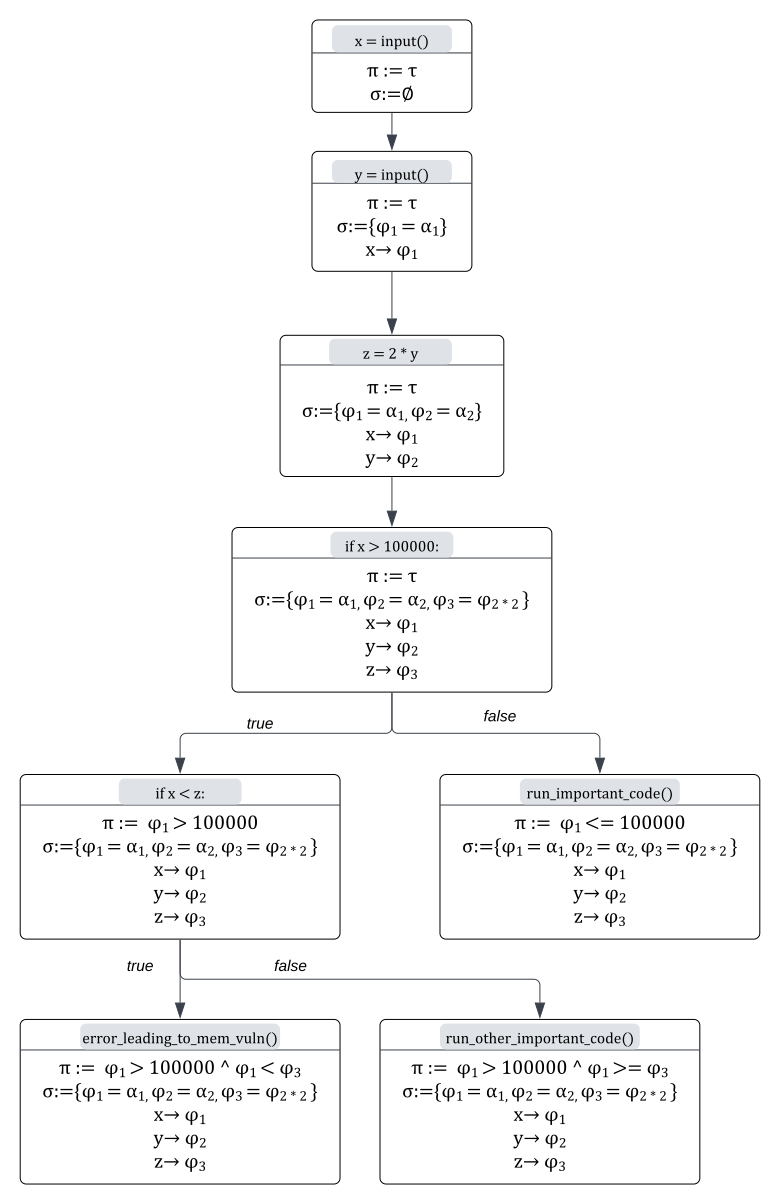
\includegraphics[scale=0.31]{figures/final_symbolic_example_graph.png}
        \caption{} % används för rendera b) som caption
        \label{fig:symbex_example_graph}
    \end{subfigure}

    \caption{Exempel för att visa symbolisk exekvering: pseudokod (a) och path
        constraint och symboliskt tillstånd för alla vägar i pseudokoden angett
        i (b). $  \mathcal{S} = \{\sigma := \{\phi_1 = \alpha_1, \phi_2 = \alpha_2, \phi_3 =
            2\phi_2\}, x \rightarrow \phi_1, y \rightarrow \phi_2, z \rightarrow
            \phi_3\}$}
\end{figure}

Exempelprogrammet i figur~\ref{fig:symbex_example_code} använder symbolisk
exekvering för att hitta vilken indata som leder programexekveringen till de
olika grenarna i programflödet. I många fall är det intressant att göra en
uttömmande sökning och hitta alla möjliga vägar i ett program, något som är
möjligt i detta program men inte i alla. Ett motexempel är komplexa
program som på grund av vägexplosionsproblemet inte hittar alla möjliga vägar.
Variablerna \emph{x} och \emph{y} sätts till symboliska värden som sedan används
för att beräkna vägvillkoret och de symboliska uttryck som variablerna utvecklas
till för en vald gren. Därefter används dessa uttryck och vägvillkor 
tillsammans för att bilda en ekvation som sedan kan lösas med hjälp av en SMT-lösare.
Figur~\ref{fig:symbex_example_graph} visar
hur det symboliska tillståndet förändras för alla möjliga grenar i programmet.

I~\ref{fig:symbex_example_graph} används $\pi$ för att ange vägvillkoret vilket
är initialt satt till $\top$ eftersom villkoret är sant från början och $\sigma$
används för att visa mappningen för symboliska värden. $\pi$ och $\sigma$ % något man kan använda ist för mappning kanske
populeras längs med exekveringen, och \emph{x} och \emph{y} mappas till
symboliska värden. Beroende på vilken väg som väljs i exekveringen, uppdateras
vägvillkoret. I andra noden sett uppifrån finns det två skillnader i jämförelse
med den första noden: \emph{x} tilldelas $\phi_1$ som är en symbolisk mappning
till $\alpha_1$. Efter den fjärde noden sett uppifrån görs ett val och
vägvillkoret förändras beroende på vilken väg som tas -- vägvillkoret uppdateras
till $\phi_1 > 100000$ om $x < z$ och annars uppdateras det till $\phi_1 \leq 
    100000$. På samma sätt uppdateras $\pi$ och $\phi$ längs andra exekveringsvägar
och vilket till slut leder till ett komplett programflödesdiagram som beror på
\emph{x, y, z}. I varje nod kan ett konkret värde som uppfyller vägvillkoren evalueras.

\section{Statisk och dynamisk binäranalys}
En annan typ av kategorisering av olika analysmetoder som fokuserar på hur
analysen genomförs delar metoderna i två grupper: statisk och dynamisk
analys~\cite{dynamic_bin_analysis}.

Statisk analys syftar på analys som går att göra utan att exekvera programmet
som analyseras. Exempel på statisk binäranalys är metod 1--2, alltså att
disassembla binären och/eller visualisera kod~\cite{dynamic_bin_analysis}.

Dynamisk analys går ut på att analysera ett program under
exekvering~\cite{dynamic_bin_analysis}. Exempel på dynamisk binäranalys är
metod 3--6. I alla fall krävs någon typ av injektion av kod eller data i
programmet i syfte att kunna extrahera viktig information under programmets
körning~\cite{dynamic_bin_analysis}. Många avancerade dynamiska metoder som
t.ex.\ concolic testing kräver symbolisk exekvering som går ut på att tilldela
symboliska värden till variabler och se hur dessa påverkar programhopp och
förgreningar och vad för möjliga värden som denna symbol kan inneha under
exekvering. I fallet med concolic testing används denna information för att,
med hjälp av en SMT-solver ta fram konkreta värden som leder till att
programmet kör till en program-distination som består av ett krasch.

\section{Arkitektur för binäranalysverktyg}

Kärnan i ett korrekt dynamisk binäranalysverktyg är en \emph{exekveringsmotor},
en komponent som på ett korrekt vis kan exekvera programmet.
Figur~\ref{schematic} visar förhållandet mellan användaren, analysverktyget och
dess exekveringsmotor. Att köra ett program innebär att ladda binären och dess
bibliotek, hoppa till startadressen och sedan köra enskilda instruktioner. Om
binäranalysverktyget ska kunna använda metoder som använder symbolisk
exekvering behöver denna exekvering av enskilda instruktioner också stödja
symboliska variabler.


\begin{figure}[H]
    \centering
    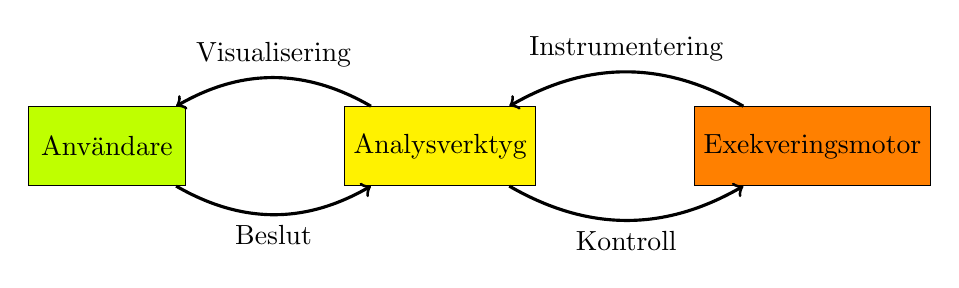
\begin{tikzpicture}

        \node [draw, fill=lime, minimum
            width=2cm, minimum height=1cm, ]  (user) {Användare};

        \node [draw, fill=yellow, minimum width=2cm, minimum height=1cm,
            right=2cm of user ] (tool) {Analysverktyg};

        \node [draw, fill=orange, minimum width=2cm, minimum height=1cm,
            right=2cm of tool ] (engine) {Exekveringsmotor};

        \draw[->, line width=.4mm] (user.-30) to[out=-30, in=-150]
        node[midway,below]{Beslut} (tool.-150);

        \draw[->, line width=.4mm] (tool.150) to[out=150, in=30]
        node[midway,above]{Visualisering} (user.30);

        \draw[->, line width=.4mm] (tool.-30) to[out=-30, in=-150]
        node[midway,below]{Kontroll} (engine.-150);

        \draw[->, line width=.4mm] (engine.150) to[out=150, in=30]
        node[midway,above]{Instrumentering} (tool.30);

    \end{tikzpicture}
    \caption{ Schematisk bild av ett binäranalysverktyg byggt kring en exekveringsmotor}\label{schematic}
\end{figure}

Symbolisk exekvering innehar, i praktiken, begränsningar i skalbarhet. En
symbolisk exekveringsmotor som utför symbolisk exekvering behöver ta hänsyn
till ett antal frågor gällande~\cite{survey_symb_exc}:

\paragraph{Minne} Motorn behöver spara komplexa datatyper och representera de
på ett sätt som tillåter villkorslösning. Exekvering av större program kräver
mer minne för att bokföra symboler och uttryck och därmed mer tid för
exekvering~\cite{survey_symb_exc}.

\paragraph{Miljö} Program i verkligheten kommunicerar på många sätt med sin
omgivning. För program är detta en virtuell miljö bestående av filer,
biblioteksanrop och IPC (\emph{inter process communication}). För att en
\textit{exekveringsmotor} ska vara så brett tillämpbar som möjligt behöver den
också stödja flera sorters omgivningskommunikation och representera omgivningen
på ett så komplett sätt som möjligt~\cite{survey_symb_exc}.

\paragraph{Stigexplotion} Verkliga program innehåller loopar, rekursion,
undantag och kombinationer av dessa som kan orsaka ett exponentiellt ökande
antal exekveringsvägar i programflödet. Det är alltså osannolikt att en motor
kan uttömmande utforska alla möjliga exekveringsvägar inom rimlig tid.
\emph{State-merging} kan appliceras i vissa fall för att begränsa antal
exekveringsvägar. \emph{State-merging} går ut på att slå samman ett antal
exekveringsvägar genom att upptäcka exekveringsvägar som liknar varandra och
slå samman dessa genom att kombinera dess villkor. Det krävs heuristik för att
upptäcka fall där \emph{state-merging} är applicerbart~\cite{survey_symb_exc}.

\paragraph{Villkorslösning} SMT-lösare kan skala till komplexa kombinationer av
villkor över hundratals variabler. Däremot kan icke-linjär aritmetik utgöra ett
stort hinder för effektivitet. Dessutom finns det exempel på olösliga problem
där SMT-lösare är inte tillämpbara~\cite{survey_symb_exc}.

% \subsection{Analyser}
%
% Det finns många möjliga analyser som kan användas av ett binäranalysverktyg, där
% \textit{analyser} avser en visualisering av en aspekt av det analyserade
% programmets beteende eventuellt inklusive ett sätt för användaren att påverka
% det analyserade programmets körning.
%
% En konkret exekvering kan spåras och dess instruktionssekvens kan visas för
% användaren med loopar identifierade. Flera exekveringar kan visualiseras på
% samma sätt och deras instruktionssekvenser användas för att återskapa
% kontrollflödesstrukturer som for- och while-loopar och if-satser.
%
% Möjligheter för \textit{state merging} kan identifieras helautomatiskt eller av
% användaren, alltså platser där flera exekveringar kan ersättas av en enda mer
% generell exekvering som innehåller ursprungsexekveringarnas skillnader som
% symboliska uttryck.
%
% En uppsättning liknande exekveringar kan visas upp för användaren tillsammans
% med information om när och hur de divergerar, för att till exempel avgöra när
% olika delar av indatan används.
%
% För analys av programmet är det också hjälpsamt för användaren att kunna stega
% genom exekveringen steg för steg och ändra på värden för att ta de vägar de vill
% analysera. Detta borde också kunna göras baklänges, det vill säga att användaren
% väljer en slutdestination och låter programmet själv lista ut vilka värden som
% behövdes läsas för att exekveringen skulle ta sig till den punkten.
%
% En mer automatisk men ändå viktig funktionalitet är konstruktion av kod-täckande
% indata. När testfall som besöker en uppsättning instruktioner är konstruerad kan
% kraven på indatan över denna uppsättning programhopp analyseras och programmet
% kan lista ut vilka aspekter av indatan som kan ändras utan att påverka
% kodtäckningsgraden, och kommunicera detta till användaren.
%
% Det finns många möjliga analyser. Användbarheten i ett verktyg mäts inte i
% kvantiteten analyser utan i förmågan för de utvalda implementerade analyserna
% att täcka användarens behov av förståelse av programmet.


\chapter{Existerande verktyg}
För att evaluera verktyget används existerande verktyg som jämförelse i
kombination med att dess fördelar och nackdelar vägs mot AMBA. Dessutom
presenteras en diskussion kring utvecklingsprocessens gång och
vidareutvecklingspotential.

\section{Jämförelse mellan AMBA och Ghidra} Ghidra är ett avancerat verktyg som
gör statisk analys bortom syftet med AMBA, men AMBA har ett par likheter. Ghidra
kan representera en kontrollflödesgraf för en given binär på två olika sätt:
\textit{Flow Graph} och \textit{Code Flow Graph}~\cite{ghidra_website}.

\begin{figure}[H]
    \begin{subfigure}{0.3\textwidth}
        \includegraphics[width=\linewidth]{figures/ghidra_code_listing.png}
        \caption{Ghidras code listing.} \label{fig:ghidra_code_listing}
    \end{subfigure}
    \hspace*{\fill}
    \begin{subfigure}{0.3\textwidth}
        \includegraphics[width=\linewidth]{figures/ghidra_block_flow_graph.png}
        \caption{Ghidras block-flow-graph.}
        \label{fig:ghidra_block_graph}
    \end{subfigure}
    \hspace*{\fill}
    \begin{subfigure}{0.3\textwidth}
        \includegraphics[width=\linewidth]{figures/ghidra_code_flow.png}
        \caption{Ghidras code-flow-graph.} \label{fig:ghidra_code_flow_graph}
    \end{subfigure}

    \caption{Tre primära vyer i verktyget Ghidra för att representera ett programs
        kontrollflödesgraf.} \label{fig:ghidra_figures}
\end{figure}

Ghidra kompletterar dessa vyer med en \textit{code listing}, en primär vy där
binärens disassemblerade kod listas. Användaren kan fritt välja att bilda en
graf från ett markerat \textit{code block}, vilket är Ghidras utökade
specifikation på ett basic block, från Ghidras code
listing~\cite{ghidra_website}. AMBA har liknande funktionalitet, se
figur~\ref{fig:graf-basic}, och kan visualisera binärens fullständiga
disassemblerade kod för en given nod, om debugdata finns tillgänglig, men saknar
större kontext likt Ghidras code listing. En fördel mot Ghidras representation
är AMBAs tre olika sätt att representera en binärs kontrollflöde på: \textit{Raw
    Basic Block Graph}, \textit{Compressed Block Graph}, och \textit{State Graph}.
Genom att använda dessa tre olika vyer kan en användare bilda en större
förståelse om en given binär, dels genom att exempelvis visualisera alla
symboliska tillstånd som \stoe{} skapar i kombination med färgade noder som
indikerar på starkt kopplade komponenter (jfr. eng. \emph{strongly connected
    components}).

Kännedom om starkt kopplade komponenter i en kontrollflödesgraf är i synnerhet
intressant vid analys av binärer utan källkod, eftersom dessa delgrafer speglar
en starkare koppling mellan noderna och indikerar på en sektion i binären som
troligtvis har större relevans än en sektion som saknar eller har betydligt
färre starkt kopplade komponenter. Ett typiskt mönster man kan se med starkt
kopplade komponenter är icke-nestlade loopar.

En användare skulle exempelvis kunna använda AMBAs node colouring för att bilda
en större uppfattning om en viss del i binären och sedan komplettera med
nodernas minnesaddresser för att visualisera samma sektion i ett mer avancerat
verktyg som Ghidra. Ett typiskt användningsfall skulle kunna vara att i Ghidra
söka efter strängar som ger mer information i den givna kodsektionen från AMBA
eller använda Ghidras analysmetoder för att dekompilera binärens instruktioner
till ett mer läsbart format i form av pseudokod.

\section{Jämförelse mellan S2E och Angr som \\ backend} Eftersom AMBA använder
\stoe{} som symbolisk exekveringsmotor har AMBA således en teoretisk fördel i
prestanda, något som kan avläsas från figurerna
i~\cite[Figur~1-5]{systematic_comparison_symbex}. Delvis beror detta på att Angr
är skrivet i python som är ett interpreterat språk och \stoe{} som är skrivet i
C++ som är ett kompilerat språk. Detta innebär att AMBA inte nödvändigtvis i
nuläget har bättre prestanda mot applikationer utvecklade med Angr som
\emph{backend}. Dock betyder det att AMBA har en teoretisk konkurrenskraftig
prestanda.

Angr är dock ett mer flexibelt verktyg som har den funktionalitet som \stoe{}
tillhandahåller, och är dessutom i allmänhet enklare att påbörja utveckling med
och onekligen eklare att bygga. Dessutom är Angr i synnerhet ett eftertraktat
verktyg att använda som symbolisk exekveringsmotor eftersom det bland annat
tillhandahåller funktionalitet såsom \emph{Control-Flow Graph Recovery} och
disassemblering som möjliggör mycket av funktionalitet som annars behövdes
implementeras i AMBA.

\section{Jämförelse mellan AMBA och SymNav} SymNav tillhandahåller samma
funktionalitet som AMBA gör bortsett från en detalj: användare kan genom SymNav
ta bort states som inte är intressanta medan i AMBA kan användare prioritera
states som ska analyseras. Dessutom presenteras funktionaliteten i SymNav på ett
mer användarvänligt sätt: vyn splittar upp respektive funktionalitet i
applikationen och presenterar detta i stil med designmönstret \emph{Grid of
    equals}.

Utöver detta är den stora skillnaden vilken symbolisk exekveringsmotor som
används. SymNav använder Angr, och AMBA använder, som tidigare nämnt, \stoe{}
vilket innebär att SymNav får en enklare kodbas eftersom mycket av koden som
interagerar med Angr är pythonskript likt API-anrop vilket kräver mindre total
kod för att uppnå samma sak som med \stoe{} men är istället begränsad i
skalbarhet. \stoe{} har inbyggda plugins som tillhandahåller mycket
funktionalitet, till exempel \emph{ExecutionTracer} som övervakar och
registrerar information längs med exekveringen för en given branch vilket
tillåter en att undersöka vad som orsakar path explosion eller vilken branch som
gör flest förgreningar.

\section{Arbetsprocess}
Eftersom \stoe{} är ett komplext system med många komplicerade
biblioteksberoenden ansågs det tidigt i arbetsprocessen att göra AMBA mer
tillgängligt till slutanvändaren genom att paketera alla bibliotek som krävs för
att köra \stoe{}. Detta var en komplicerad och tidskrävande uppgift eftersom
mycket av \stoe{}s byggsystem var tvunget att återimplementeras eller kringgås
när tvetydiga och icke-triviala problem uppstod. Ett sådant problem var
nedladdningen och byggningen av guest images som \stoe{} lagrades på google
drive där lösningen var att istället ladda ner färdiga guest images.

Denna del av arbetet ledde till att mycket av planeringen blev förskjutet och
således fanns det mindre tid till att utveckla all funktionalitet som var tänkt.

\section{Vidareutveckling}
En särskilt eftertraktad funktionalitet är \textit{State merging}. Syftet med
state merging är att minska antalet exekveringsvägar genom att förena symboliska
tillstånd som är ekvivalenta. Genom att introducera state merging ökar
prestandan för den symboliska exekveringen som gör det möjligt att skicka fler
förfrågningar (jfr. eng. \emph{queries}) till SMT-lösaren.

Övervakning av systemanrop (jfr. eng. \emph{syscalls}) ger användaren en större
insikt i vad som sker i en specifik del av grafen, exempelvis om det sker
inmatning eller utmatning, om en process signaleras att stängas av, om binären
kör ett exec-systemanrop för att köra ett externt program, etc. är anledningar
som gör det intressant att övervaka systemanrop. För att implementera detta i
AMBA bör det undersökas om det finns hooks för detta.

I nuläget sparas inte resultatet från SMT-lösaren för ett givet path constraint
och därför får användaren inte heller mer informatiom om vilken input som ledde
till att vägen nåddes i exekveringen. Optimalt hade varit om användaren kunde se
vilken indata som ledde till en särskild väg för fortsatt analys. \stoe{} har
denna information, men i nuläget sparas den inte av AMBA.



\chapter{AMBA}
För att evaluera verktyget används existerande verktyg som jämförelse i
kombination med att dess fördelar och nackdelar vägs mot AMBA. Dessutom
presenteras en diskussion kring utvecklingsprocessens gång och
vidareutvecklingspotential.

\section{Jämförelse mellan AMBA och Ghidra} Ghidra är ett avancerat verktyg som
gör statisk analys bortom syftet med AMBA, men AMBA har ett par likheter. Ghidra
kan representera en kontrollflödesgraf för en given binär på två olika sätt:
\textit{Flow Graph} och \textit{Code Flow Graph}~\cite{ghidra_website}.

\begin{figure}[H]
    \begin{subfigure}{0.3\textwidth}
        \includegraphics[width=\linewidth]{figures/ghidra_code_listing.png}
        \caption{Ghidras code listing.} \label{fig:ghidra_code_listing}
    \end{subfigure}
    \hspace*{\fill}
    \begin{subfigure}{0.3\textwidth}
        \includegraphics[width=\linewidth]{figures/ghidra_block_flow_graph.png}
        \caption{Ghidras block-flow-graph.}
        \label{fig:ghidra_block_graph}
    \end{subfigure}
    \hspace*{\fill}
    \begin{subfigure}{0.3\textwidth}
        \includegraphics[width=\linewidth]{figures/ghidra_code_flow.png}
        \caption{Ghidras code-flow-graph.} \label{fig:ghidra_code_flow_graph}
    \end{subfigure}

    \caption{Tre primära vyer i verktyget Ghidra för att representera ett programs
        kontrollflödesgraf.} \label{fig:ghidra_figures}
\end{figure}

Ghidra kompletterar dessa vyer med en \textit{code listing}, en primär vy där
binärens disassemblerade kod listas. Användaren kan fritt välja att bilda en
graf från ett markerat \textit{code block}, vilket är Ghidras utökade
specifikation på ett basic block, från Ghidras code
listing~\cite{ghidra_website}. AMBA har liknande funktionalitet, se
figur~\ref{fig:graf-basic}, och kan visualisera binärens fullständiga
disassemblerade kod för en given nod, om debugdata finns tillgänglig, men saknar
större kontext likt Ghidras code listing. En fördel mot Ghidras representation
är AMBAs tre olika sätt att representera en binärs kontrollflöde på: \textit{Raw
    Basic Block Graph}, \textit{Compressed Block Graph}, och \textit{State Graph}.
Genom att använda dessa tre olika vyer kan en användare bilda en större
förståelse om en given binär, dels genom att exempelvis visualisera alla
symboliska tillstånd som \stoe{} skapar i kombination med färgade noder som
indikerar på starkt kopplade komponenter (jfr. eng. \emph{strongly connected
    components}).

Kännedom om starkt kopplade komponenter i en kontrollflödesgraf är i synnerhet
intressant vid analys av binärer utan källkod, eftersom dessa delgrafer speglar
en starkare koppling mellan noderna och indikerar på en sektion i binären som
troligtvis har större relevans än en sektion som saknar eller har betydligt
färre starkt kopplade komponenter. Ett typiskt mönster man kan se med starkt
kopplade komponenter är icke-nestlade loopar.

En användare skulle exempelvis kunna använda AMBAs node colouring för att bilda
en större uppfattning om en viss del i binären och sedan komplettera med
nodernas minnesaddresser för att visualisera samma sektion i ett mer avancerat
verktyg som Ghidra. Ett typiskt användningsfall skulle kunna vara att i Ghidra
söka efter strängar som ger mer information i den givna kodsektionen från AMBA
eller använda Ghidras analysmetoder för att dekompilera binärens instruktioner
till ett mer läsbart format i form av pseudokod.

\section{Jämförelse mellan S2E och Angr som \\ backend} Eftersom AMBA använder
\stoe{} som symbolisk exekveringsmotor har AMBA således en teoretisk fördel i
prestanda, något som kan avläsas från figurerna
i~\cite[Figur~1-5]{systematic_comparison_symbex}. Delvis beror detta på att Angr
är skrivet i python som är ett interpreterat språk och \stoe{} som är skrivet i
C++ som är ett kompilerat språk. Detta innebär att AMBA inte nödvändigtvis i
nuläget har bättre prestanda mot applikationer utvecklade med Angr som
\emph{backend}. Dock betyder det att AMBA har en teoretisk konkurrenskraftig
prestanda.

Angr är dock ett mer flexibelt verktyg som har den funktionalitet som \stoe{}
tillhandahåller, och är dessutom i allmänhet enklare att påbörja utveckling med
och onekligen eklare att bygga. Dessutom är Angr i synnerhet ett eftertraktat
verktyg att använda som symbolisk exekveringsmotor eftersom det bland annat
tillhandahåller funktionalitet såsom \emph{Control-Flow Graph Recovery} och
disassemblering som möjliggör mycket av funktionalitet som annars behövdes
implementeras i AMBA.

\section{Jämförelse mellan AMBA och SymNav} SymNav tillhandahåller samma
funktionalitet som AMBA gör bortsett från en detalj: användare kan genom SymNav
ta bort states som inte är intressanta medan i AMBA kan användare prioritera
states som ska analyseras. Dessutom presenteras funktionaliteten i SymNav på ett
mer användarvänligt sätt: vyn splittar upp respektive funktionalitet i
applikationen och presenterar detta i stil med designmönstret \emph{Grid of
    equals}.

Utöver detta är den stora skillnaden vilken symbolisk exekveringsmotor som
används. SymNav använder Angr, och AMBA använder, som tidigare nämnt, \stoe{}
vilket innebär att SymNav får en enklare kodbas eftersom mycket av koden som
interagerar med Angr är pythonskript likt API-anrop vilket kräver mindre total
kod för att uppnå samma sak som med \stoe{} men är istället begränsad i
skalbarhet. \stoe{} har inbyggda plugins som tillhandahåller mycket
funktionalitet, till exempel \emph{ExecutionTracer} som övervakar och
registrerar information längs med exekveringen för en given branch vilket
tillåter en att undersöka vad som orsakar path explosion eller vilken branch som
gör flest förgreningar.

\section{Arbetsprocess}
Eftersom \stoe{} är ett komplext system med många komplicerade
biblioteksberoenden ansågs det tidigt i arbetsprocessen att göra AMBA mer
tillgängligt till slutanvändaren genom att paketera alla bibliotek som krävs för
att köra \stoe{}. Detta var en komplicerad och tidskrävande uppgift eftersom
mycket av \stoe{}s byggsystem var tvunget att återimplementeras eller kringgås
när tvetydiga och icke-triviala problem uppstod. Ett sådant problem var
nedladdningen och byggningen av guest images som \stoe{} lagrades på google
drive där lösningen var att istället ladda ner färdiga guest images.

Denna del av arbetet ledde till att mycket av planeringen blev förskjutet och
således fanns det mindre tid till att utveckla all funktionalitet som var tänkt.

\section{Vidareutveckling}
En särskilt eftertraktad funktionalitet är \textit{State merging}. Syftet med
state merging är att minska antalet exekveringsvägar genom att förena symboliska
tillstånd som är ekvivalenta. Genom att introducera state merging ökar
prestandan för den symboliska exekveringen som gör det möjligt att skicka fler
förfrågningar (jfr. eng. \emph{queries}) till SMT-lösaren.

Övervakning av systemanrop (jfr. eng. \emph{syscalls}) ger användaren en större
insikt i vad som sker i en specifik del av grafen, exempelvis om det sker
inmatning eller utmatning, om en process signaleras att stängas av, om binären
kör ett exec-systemanrop för att köra ett externt program, etc. är anledningar
som gör det intressant att övervaka systemanrop. För att implementera detta i
AMBA bör det undersökas om det finns hooks för detta.

I nuläget sparas inte resultatet från SMT-lösaren för ett givet path constraint
och därför får användaren inte heller mer informatiom om vilken input som ledde
till att vägen nåddes i exekveringen. Optimalt hade varit om användaren kunde se
vilken indata som ledde till en särskild väg för fortsatt analys. \stoe{} har
denna information, men i nuläget sparas den inte av AMBA.



\chapter{Implementation}
För att evaluera verktyget används existerande verktyg som jämförelse i
kombination med att dess fördelar och nackdelar vägs mot AMBA. Dessutom
presenteras en diskussion kring utvecklingsprocessens gång och
vidareutvecklingspotential.

\section{Jämförelse mellan AMBA och Ghidra} Ghidra är ett avancerat verktyg som
gör statisk analys bortom syftet med AMBA, men AMBA har ett par likheter. Ghidra
kan representera en kontrollflödesgraf för en given binär på två olika sätt:
\textit{Flow Graph} och \textit{Code Flow Graph}~\cite{ghidra_website}.

\begin{figure}[H]
    \begin{subfigure}{0.3\textwidth}
        \includegraphics[width=\linewidth]{figures/ghidra_code_listing.png}
        \caption{Ghidras code listing.} \label{fig:ghidra_code_listing}
    \end{subfigure}
    \hspace*{\fill}
    \begin{subfigure}{0.3\textwidth}
        \includegraphics[width=\linewidth]{figures/ghidra_block_flow_graph.png}
        \caption{Ghidras block-flow-graph.}
        \label{fig:ghidra_block_graph}
    \end{subfigure}
    \hspace*{\fill}
    \begin{subfigure}{0.3\textwidth}
        \includegraphics[width=\linewidth]{figures/ghidra_code_flow.png}
        \caption{Ghidras code-flow-graph.} \label{fig:ghidra_code_flow_graph}
    \end{subfigure}

    \caption{Tre primära vyer i verktyget Ghidra för att representera ett programs
        kontrollflödesgraf.} \label{fig:ghidra_figures}
\end{figure}

Ghidra kompletterar dessa vyer med en \textit{code listing}, en primär vy där
binärens disassemblerade kod listas. Användaren kan fritt välja att bilda en
graf från ett markerat \textit{code block}, vilket är Ghidras utökade
specifikation på ett basic block, från Ghidras code
listing~\cite{ghidra_website}. AMBA har liknande funktionalitet, se
figur~\ref{fig:graf-basic}, och kan visualisera binärens fullständiga
disassemblerade kod för en given nod, om debugdata finns tillgänglig, men saknar
större kontext likt Ghidras code listing. En fördel mot Ghidras representation
är AMBAs tre olika sätt att representera en binärs kontrollflöde på: \textit{Raw
    Basic Block Graph}, \textit{Compressed Block Graph}, och \textit{State Graph}.
Genom att använda dessa tre olika vyer kan en användare bilda en större
förståelse om en given binär, dels genom att exempelvis visualisera alla
symboliska tillstånd som \stoe{} skapar i kombination med färgade noder som
indikerar på starkt kopplade komponenter (jfr. eng. \emph{strongly connected
    components}).

Kännedom om starkt kopplade komponenter i en kontrollflödesgraf är i synnerhet
intressant vid analys av binärer utan källkod, eftersom dessa delgrafer speglar
en starkare koppling mellan noderna och indikerar på en sektion i binären som
troligtvis har större relevans än en sektion som saknar eller har betydligt
färre starkt kopplade komponenter. Ett typiskt mönster man kan se med starkt
kopplade komponenter är icke-nestlade loopar.

En användare skulle exempelvis kunna använda AMBAs node colouring för att bilda
en större uppfattning om en viss del i binären och sedan komplettera med
nodernas minnesaddresser för att visualisera samma sektion i ett mer avancerat
verktyg som Ghidra. Ett typiskt användningsfall skulle kunna vara att i Ghidra
söka efter strängar som ger mer information i den givna kodsektionen från AMBA
eller använda Ghidras analysmetoder för att dekompilera binärens instruktioner
till ett mer läsbart format i form av pseudokod.

\section{Jämförelse mellan S2E och Angr som \\ backend} Eftersom AMBA använder
\stoe{} som symbolisk exekveringsmotor har AMBA således en teoretisk fördel i
prestanda, något som kan avläsas från figurerna
i~\cite[Figur~1-5]{systematic_comparison_symbex}. Delvis beror detta på att Angr
är skrivet i python som är ett interpreterat språk och \stoe{} som är skrivet i
C++ som är ett kompilerat språk. Detta innebär att AMBA inte nödvändigtvis i
nuläget har bättre prestanda mot applikationer utvecklade med Angr som
\emph{backend}. Dock betyder det att AMBA har en teoretisk konkurrenskraftig
prestanda.

Angr är dock ett mer flexibelt verktyg som har den funktionalitet som \stoe{}
tillhandahåller, och är dessutom i allmänhet enklare att påbörja utveckling med
och onekligen eklare att bygga. Dessutom är Angr i synnerhet ett eftertraktat
verktyg att använda som symbolisk exekveringsmotor eftersom det bland annat
tillhandahåller funktionalitet såsom \emph{Control-Flow Graph Recovery} och
disassemblering som möjliggör mycket av funktionalitet som annars behövdes
implementeras i AMBA.

\section{Jämförelse mellan AMBA och SymNav} SymNav tillhandahåller samma
funktionalitet som AMBA gör bortsett från en detalj: användare kan genom SymNav
ta bort states som inte är intressanta medan i AMBA kan användare prioritera
states som ska analyseras. Dessutom presenteras funktionaliteten i SymNav på ett
mer användarvänligt sätt: vyn splittar upp respektive funktionalitet i
applikationen och presenterar detta i stil med designmönstret \emph{Grid of
    equals}.

Utöver detta är den stora skillnaden vilken symbolisk exekveringsmotor som
används. SymNav använder Angr, och AMBA använder, som tidigare nämnt, \stoe{}
vilket innebär att SymNav får en enklare kodbas eftersom mycket av koden som
interagerar med Angr är pythonskript likt API-anrop vilket kräver mindre total
kod för att uppnå samma sak som med \stoe{} men är istället begränsad i
skalbarhet. \stoe{} har inbyggda plugins som tillhandahåller mycket
funktionalitet, till exempel \emph{ExecutionTracer} som övervakar och
registrerar information längs med exekveringen för en given branch vilket
tillåter en att undersöka vad som orsakar path explosion eller vilken branch som
gör flest förgreningar.

\section{Arbetsprocess}
Eftersom \stoe{} är ett komplext system med många komplicerade
biblioteksberoenden ansågs det tidigt i arbetsprocessen att göra AMBA mer
tillgängligt till slutanvändaren genom att paketera alla bibliotek som krävs för
att köra \stoe{}. Detta var en komplicerad och tidskrävande uppgift eftersom
mycket av \stoe{}s byggsystem var tvunget att återimplementeras eller kringgås
när tvetydiga och icke-triviala problem uppstod. Ett sådant problem var
nedladdningen och byggningen av guest images som \stoe{} lagrades på google
drive där lösningen var att istället ladda ner färdiga guest images.

Denna del av arbetet ledde till att mycket av planeringen blev förskjutet och
således fanns det mindre tid till att utveckla all funktionalitet som var tänkt.

\section{Vidareutveckling}
En särskilt eftertraktad funktionalitet är \textit{State merging}. Syftet med
state merging är att minska antalet exekveringsvägar genom att förena symboliska
tillstånd som är ekvivalenta. Genom att introducera state merging ökar
prestandan för den symboliska exekveringen som gör det möjligt att skicka fler
förfrågningar (jfr. eng. \emph{queries}) till SMT-lösaren.

Övervakning av systemanrop (jfr. eng. \emph{syscalls}) ger användaren en större
insikt i vad som sker i en specifik del av grafen, exempelvis om det sker
inmatning eller utmatning, om en process signaleras att stängas av, om binären
kör ett exec-systemanrop för att köra ett externt program, etc. är anledningar
som gör det intressant att övervaka systemanrop. För att implementera detta i
AMBA bör det undersökas om det finns hooks för detta.

I nuläget sparas inte resultatet från SMT-lösaren för ett givet path constraint
och därför får användaren inte heller mer informatiom om vilken input som ledde
till att vägen nåddes i exekveringen. Optimalt hade varit om användaren kunde se
vilken indata som ledde till en särskild väg för fortsatt analys. \stoe{} har
denna information, men i nuläget sparas den inte av AMBA.



\chapter{Evaluering}
För att evaluera verktyget används existerande verktyg som jämförelse i
kombination med att dess fördelar och nackdelar vägs mot AMBA. Dessutom
presenteras en diskussion kring utvecklingsprocessens gång och
vidareutvecklingspotential.

\section{Jämförelse mellan AMBA och Ghidra} Ghidra är ett avancerat verktyg som
gör statisk analys bortom syftet med AMBA, men AMBA har ett par likheter. Ghidra
kan representera en kontrollflödesgraf för en given binär på två olika sätt:
\textit{Flow Graph} och \textit{Code Flow Graph}~\cite{ghidra_website}.

\begin{figure}[H]
    \begin{subfigure}{0.3\textwidth}
        \includegraphics[width=\linewidth]{figures/ghidra_code_listing.png}
        \caption{Ghidras code listing.} \label{fig:ghidra_code_listing}
    \end{subfigure}
    \hspace*{\fill}
    \begin{subfigure}{0.3\textwidth}
        \includegraphics[width=\linewidth]{figures/ghidra_block_flow_graph.png}
        \caption{Ghidras block-flow-graph.}
        \label{fig:ghidra_block_graph}
    \end{subfigure}
    \hspace*{\fill}
    \begin{subfigure}{0.3\textwidth}
        \includegraphics[width=\linewidth]{figures/ghidra_code_flow.png}
        \caption{Ghidras code-flow-graph.} \label{fig:ghidra_code_flow_graph}
    \end{subfigure}

    \caption{Tre primära vyer i verktyget Ghidra för att representera ett programs
        kontrollflödesgraf.} \label{fig:ghidra_figures}
\end{figure}

Ghidra kompletterar dessa vyer med en \textit{code listing}, en primär vy där
binärens disassemblerade kod listas. Användaren kan fritt välja att bilda en
graf från ett markerat \textit{code block}, vilket är Ghidras utökade
specifikation på ett basic block, från Ghidras code
listing~\cite{ghidra_website}. AMBA har liknande funktionalitet, se
figur~\ref{fig:graf-basic}, och kan visualisera binärens fullständiga
disassemblerade kod för en given nod, om debugdata finns tillgänglig, men saknar
större kontext likt Ghidras code listing. En fördel mot Ghidras representation
är AMBAs tre olika sätt att representera en binärs kontrollflöde på: \textit{Raw
    Basic Block Graph}, \textit{Compressed Block Graph}, och \textit{State Graph}.
Genom att använda dessa tre olika vyer kan en användare bilda en större
förståelse om en given binär, dels genom att exempelvis visualisera alla
symboliska tillstånd som \stoe{} skapar i kombination med färgade noder som
indikerar på starkt kopplade komponenter (jfr. eng. \emph{strongly connected
    components}).

Kännedom om starkt kopplade komponenter i en kontrollflödesgraf är i synnerhet
intressant vid analys av binärer utan källkod, eftersom dessa delgrafer speglar
en starkare koppling mellan noderna och indikerar på en sektion i binären som
troligtvis har större relevans än en sektion som saknar eller har betydligt
färre starkt kopplade komponenter. Ett typiskt mönster man kan se med starkt
kopplade komponenter är icke-nestlade loopar.

En användare skulle exempelvis kunna använda AMBAs node colouring för att bilda
en större uppfattning om en viss del i binären och sedan komplettera med
nodernas minnesaddresser för att visualisera samma sektion i ett mer avancerat
verktyg som Ghidra. Ett typiskt användningsfall skulle kunna vara att i Ghidra
söka efter strängar som ger mer information i den givna kodsektionen från AMBA
eller använda Ghidras analysmetoder för att dekompilera binärens instruktioner
till ett mer läsbart format i form av pseudokod.

\section{Jämförelse mellan S2E och Angr som \\ backend} Eftersom AMBA använder
\stoe{} som symbolisk exekveringsmotor har AMBA således en teoretisk fördel i
prestanda, något som kan avläsas från figurerna
i~\cite[Figur~1-5]{systematic_comparison_symbex}. Delvis beror detta på att Angr
är skrivet i python som är ett interpreterat språk och \stoe{} som är skrivet i
C++ som är ett kompilerat språk. Detta innebär att AMBA inte nödvändigtvis i
nuläget har bättre prestanda mot applikationer utvecklade med Angr som
\emph{backend}. Dock betyder det att AMBA har en teoretisk konkurrenskraftig
prestanda.

Angr är dock ett mer flexibelt verktyg som har den funktionalitet som \stoe{}
tillhandahåller, och är dessutom i allmänhet enklare att påbörja utveckling med
och onekligen eklare att bygga. Dessutom är Angr i synnerhet ett eftertraktat
verktyg att använda som symbolisk exekveringsmotor eftersom det bland annat
tillhandahåller funktionalitet såsom \emph{Control-Flow Graph Recovery} och
disassemblering som möjliggör mycket av funktionalitet som annars behövdes
implementeras i AMBA.

\section{Jämförelse mellan AMBA och SymNav} SymNav tillhandahåller samma
funktionalitet som AMBA gör bortsett från en detalj: användare kan genom SymNav
ta bort states som inte är intressanta medan i AMBA kan användare prioritera
states som ska analyseras. Dessutom presenteras funktionaliteten i SymNav på ett
mer användarvänligt sätt: vyn splittar upp respektive funktionalitet i
applikationen och presenterar detta i stil med designmönstret \emph{Grid of
    equals}.

Utöver detta är den stora skillnaden vilken symbolisk exekveringsmotor som
används. SymNav använder Angr, och AMBA använder, som tidigare nämnt, \stoe{}
vilket innebär att SymNav får en enklare kodbas eftersom mycket av koden som
interagerar med Angr är pythonskript likt API-anrop vilket kräver mindre total
kod för att uppnå samma sak som med \stoe{} men är istället begränsad i
skalbarhet. \stoe{} har inbyggda plugins som tillhandahåller mycket
funktionalitet, till exempel \emph{ExecutionTracer} som övervakar och
registrerar information längs med exekveringen för en given branch vilket
tillåter en att undersöka vad som orsakar path explosion eller vilken branch som
gör flest förgreningar.

\section{Arbetsprocess}
Eftersom \stoe{} är ett komplext system med många komplicerade
biblioteksberoenden ansågs det tidigt i arbetsprocessen att göra AMBA mer
tillgängligt till slutanvändaren genom att paketera alla bibliotek som krävs för
att köra \stoe{}. Detta var en komplicerad och tidskrävande uppgift eftersom
mycket av \stoe{}s byggsystem var tvunget att återimplementeras eller kringgås
när tvetydiga och icke-triviala problem uppstod. Ett sådant problem var
nedladdningen och byggningen av guest images som \stoe{} lagrades på google
drive där lösningen var att istället ladda ner färdiga guest images.

Denna del av arbetet ledde till att mycket av planeringen blev förskjutet och
således fanns det mindre tid till att utveckla all funktionalitet som var tänkt.

\section{Vidareutveckling}
En särskilt eftertraktad funktionalitet är \textit{State merging}. Syftet med
state merging är att minska antalet exekveringsvägar genom att förena symboliska
tillstånd som är ekvivalenta. Genom att introducera state merging ökar
prestandan för den symboliska exekveringen som gör det möjligt att skicka fler
förfrågningar (jfr. eng. \emph{queries}) till SMT-lösaren.

Övervakning av systemanrop (jfr. eng. \emph{syscalls}) ger användaren en större
insikt i vad som sker i en specifik del av grafen, exempelvis om det sker
inmatning eller utmatning, om en process signaleras att stängas av, om binären
kör ett exec-systemanrop för att köra ett externt program, etc. är anledningar
som gör det intressant att övervaka systemanrop. För att implementera detta i
AMBA bör det undersökas om det finns hooks för detta.

I nuläget sparas inte resultatet från SMT-lösaren för ett givet path constraint
och därför får användaren inte heller mer informatiom om vilken input som ledde
till att vägen nåddes i exekveringen. Optimalt hade varit om användaren kunde se
vilken indata som ledde till en särskild väg för fortsatt analys. \stoe{} har
denna information, men i nuläget sparas den inte av AMBA.


\section{Metod}
\subsection{Metod}

Det är inte självklart hur utvecklingen av verktyget ska gå till och vilken 
exakt funktionalitet applikationen ska förses med för att uppfylla syftet. I det här
avsnittet beskrivs strategi, tillvägagångssätt samt evaluering av syfte i
avseende för utvecklingen.

\subsubsection{Val av strategi}

För att uppnå och redogöra för möjligheterna i en potentiell applikation
reflekterades det över två möjliga alternativ att fullfölja. Dels diskuterades
alternativet att bygga en symbolisk exekveringsmotor från grunden och fokusera
på dess tekniska detaljer och dels att använda en existerande produkt där
fokuset istället ligger på att bygga plugin vars syfte är att utöka den
existerande motorn med fler funktioner. I det senare fallet blir därmed
slutprodukten ett program som kommunicerar med ett plugin genom \stoe\ via IPC
eller liknande. 

Med syfte att göra framsteg valdes det att kolla vidare hur \stoe\ kan hjälpa i
frågan om att utöka funktionalitet i en existerande motor. \stoe\ är utvecklat
i programspråket C++ och med anledning av valet att utveckla i ett
annat programmeringsspråk, det vill säga Rust, krävs implementation av
C++-bindings. I ett första steg valdes det därför att se över hur detta går till
på lämpligt sätt och hur detta kan automatiseras med hjälp av andra verktyg
där bland annat autocxx ansågs som ett lovande alternativ.

\subsubsection{Tillvägagångssätt}

I avsikt att uppnå syftet med projektet, mer specifikt att utveckla ett
binäranalysverktyg för generella problem, bestämdes det att ta fram prototyper som ska leda det
kontinuerliga utvecklingsarbetet.

En prototyp är ett exempelprogram skapt i syfte att undersöka vilken
kapacitet verktyget har för att sedan utöka dess funktionalitet. Ett
exempelprogram ska ha som mål att visa en förmåga i verktyget som underlättar
förståelse för, eller belyser en känd intressant egenskap. Ett typiskt
intressant exempel är program som gör många programhopp, innehåller säkerhetshål
eller liknande. För att detta tillvägagångssätt ska vara genomförbart ställs
kravet att prototyperna hålls enkla samtdiigt som de uppnår sina mål.
Fortsättningsvis ska prototypen skrivas i C eftersom C-programs utseende i
binärformat relativt väl motsvarar dess källkod. Detta förenklar binäranalys och
låter prototypen fokusera på sin huvudsakliga uppgift. 

Detta tillvägagångssätt är önskvärt eftersom det tillåter att sätta uppnåbara delmål som styr
funktionalitet som ska implementeras härnäst. Prototyperna fungerar som test på dessa
funktionaliteter och visar att dessa är korrekta. Dessutom kan flera prototyper 
utvecklas samtidigt vilket tillåter parallellism inom projektarbetet och
framsteg på flera fronter.

I ett senare och/eller parallellt steg ska ett grafiskt användargränssnitt
utvecklas som tillåter användaren att traversera genom applikationen och göra
egna beslut gällande förgreningar av programmet etc. där användaren själv
bestämmer interaktivt nästa beslut som görs. Även detta arbetet styrs av
prototyper och funktionaliteter som önskas.

\subsubsection{Evaluering av syfte}

För att vidare kunna bestämma huruvida en prototyp är lämplig och ska möjliggöras
genom utvidgning av verktyget kommer följande steg användas för att evaluera hur
väl dessa tillsammans uppfyller det sammantagna syftet:

Hur väl kan prototypens analysidé kan komma att tillämpas i verktyget och hur
väl kommer analysen öka användbarhet av verktyget, kommer användas i detta
avseende. Dessutom ska det sättas i perspektiv till den tid som krävs för att
göra prototypen genomförbar med tanke på tidsramen för projektet.

Eftersom det huvudsakligen är prototyperna som styr den slutgiltiga
funktionaliteten hos verktyget är det därför även dessa som styr hur väl syftet
uppnåtts. Ett konkret sätt att mäta detta är hur generellt det slutgiltiga
verktyget blir, det vill säga går det exempelvis att definiera nya tester, som verktyget
ska kunna hantera, utan att göra ytterligare förändringar i verktyget. Dessutom,
går det att använda verktyget för generell reverse engineering eller för att lösa övningar
inom CTF?

% Hur är detta kopplat till vårt syfte? Hur uppnår vi syftet med rapporten genom
% vald metod?

% (varför är typ besvarat i val av strategi-avsnittet)

% Hur besvarar vi huruvida valet av strategi är rimligt?

%

\section{Begränsningar}
\input{evaluering/begransningar.tex}

\chapter{Slutsats}
För att evaluera verktyget används existerande verktyg som jämförelse i
kombination med att dess fördelar och nackdelar vägs mot AMBA. Dessutom
presenteras en diskussion kring utvecklingsprocessens gång och
vidareutvecklingspotential.

\section{Jämförelse mellan AMBA och Ghidra} Ghidra är ett avancerat verktyg som
gör statisk analys bortom syftet med AMBA, men AMBA har ett par likheter. Ghidra
kan representera en kontrollflödesgraf för en given binär på två olika sätt:
\textit{Flow Graph} och \textit{Code Flow Graph}~\cite{ghidra_website}.

\begin{figure}[H]
    \begin{subfigure}{0.3\textwidth}
        \includegraphics[width=\linewidth]{figures/ghidra_code_listing.png}
        \caption{Ghidras code listing.} \label{fig:ghidra_code_listing}
    \end{subfigure}
    \hspace*{\fill}
    \begin{subfigure}{0.3\textwidth}
        \includegraphics[width=\linewidth]{figures/ghidra_block_flow_graph.png}
        \caption{Ghidras block-flow-graph.}
        \label{fig:ghidra_block_graph}
    \end{subfigure}
    \hspace*{\fill}
    \begin{subfigure}{0.3\textwidth}
        \includegraphics[width=\linewidth]{figures/ghidra_code_flow.png}
        \caption{Ghidras code-flow-graph.} \label{fig:ghidra_code_flow_graph}
    \end{subfigure}

    \caption{Tre primära vyer i verktyget Ghidra för att representera ett programs
        kontrollflödesgraf.} \label{fig:ghidra_figures}
\end{figure}

Ghidra kompletterar dessa vyer med en \textit{code listing}, en primär vy där
binärens disassemblerade kod listas. Användaren kan fritt välja att bilda en
graf från ett markerat \textit{code block}, vilket är Ghidras utökade
specifikation på ett basic block, från Ghidras code
listing~\cite{ghidra_website}. AMBA har liknande funktionalitet, se
figur~\ref{fig:graf-basic}, och kan visualisera binärens fullständiga
disassemblerade kod för en given nod, om debugdata finns tillgänglig, men saknar
större kontext likt Ghidras code listing. En fördel mot Ghidras representation
är AMBAs tre olika sätt att representera en binärs kontrollflöde på: \textit{Raw
    Basic Block Graph}, \textit{Compressed Block Graph}, och \textit{State Graph}.
Genom att använda dessa tre olika vyer kan en användare bilda en större
förståelse om en given binär, dels genom att exempelvis visualisera alla
symboliska tillstånd som \stoe{} skapar i kombination med färgade noder som
indikerar på starkt kopplade komponenter (jfr. eng. \emph{strongly connected
    components}).

Kännedom om starkt kopplade komponenter i en kontrollflödesgraf är i synnerhet
intressant vid analys av binärer utan källkod, eftersom dessa delgrafer speglar
en starkare koppling mellan noderna och indikerar på en sektion i binären som
troligtvis har större relevans än en sektion som saknar eller har betydligt
färre starkt kopplade komponenter. Ett typiskt mönster man kan se med starkt
kopplade komponenter är icke-nestlade loopar.

En användare skulle exempelvis kunna använda AMBAs node colouring för att bilda
en större uppfattning om en viss del i binären och sedan komplettera med
nodernas minnesaddresser för att visualisera samma sektion i ett mer avancerat
verktyg som Ghidra. Ett typiskt användningsfall skulle kunna vara att i Ghidra
söka efter strängar som ger mer information i den givna kodsektionen från AMBA
eller använda Ghidras analysmetoder för att dekompilera binärens instruktioner
till ett mer läsbart format i form av pseudokod.

\section{Jämförelse mellan S2E och Angr som \\ backend} Eftersom AMBA använder
\stoe{} som symbolisk exekveringsmotor har AMBA således en teoretisk fördel i
prestanda, något som kan avläsas från figurerna
i~\cite[Figur~1-5]{systematic_comparison_symbex}. Delvis beror detta på att Angr
är skrivet i python som är ett interpreterat språk och \stoe{} som är skrivet i
C++ som är ett kompilerat språk. Detta innebär att AMBA inte nödvändigtvis i
nuläget har bättre prestanda mot applikationer utvecklade med Angr som
\emph{backend}. Dock betyder det att AMBA har en teoretisk konkurrenskraftig
prestanda.

Angr är dock ett mer flexibelt verktyg som har den funktionalitet som \stoe{}
tillhandahåller, och är dessutom i allmänhet enklare att påbörja utveckling med
och onekligen eklare att bygga. Dessutom är Angr i synnerhet ett eftertraktat
verktyg att använda som symbolisk exekveringsmotor eftersom det bland annat
tillhandahåller funktionalitet såsom \emph{Control-Flow Graph Recovery} och
disassemblering som möjliggör mycket av funktionalitet som annars behövdes
implementeras i AMBA.

\section{Jämförelse mellan AMBA och SymNav} SymNav tillhandahåller samma
funktionalitet som AMBA gör bortsett från en detalj: användare kan genom SymNav
ta bort states som inte är intressanta medan i AMBA kan användare prioritera
states som ska analyseras. Dessutom presenteras funktionaliteten i SymNav på ett
mer användarvänligt sätt: vyn splittar upp respektive funktionalitet i
applikationen och presenterar detta i stil med designmönstret \emph{Grid of
    equals}.

Utöver detta är den stora skillnaden vilken symbolisk exekveringsmotor som
används. SymNav använder Angr, och AMBA använder, som tidigare nämnt, \stoe{}
vilket innebär att SymNav får en enklare kodbas eftersom mycket av koden som
interagerar med Angr är pythonskript likt API-anrop vilket kräver mindre total
kod för att uppnå samma sak som med \stoe{} men är istället begränsad i
skalbarhet. \stoe{} har inbyggda plugins som tillhandahåller mycket
funktionalitet, till exempel \emph{ExecutionTracer} som övervakar och
registrerar information längs med exekveringen för en given branch vilket
tillåter en att undersöka vad som orsakar path explosion eller vilken branch som
gör flest förgreningar.

\section{Arbetsprocess}
Eftersom \stoe{} är ett komplext system med många komplicerade
biblioteksberoenden ansågs det tidigt i arbetsprocessen att göra AMBA mer
tillgängligt till slutanvändaren genom att paketera alla bibliotek som krävs för
att köra \stoe{}. Detta var en komplicerad och tidskrävande uppgift eftersom
mycket av \stoe{}s byggsystem var tvunget att återimplementeras eller kringgås
när tvetydiga och icke-triviala problem uppstod. Ett sådant problem var
nedladdningen och byggningen av guest images som \stoe{} lagrades på google
drive där lösningen var att istället ladda ner färdiga guest images.

Denna del av arbetet ledde till att mycket av planeringen blev förskjutet och
således fanns det mindre tid till att utveckla all funktionalitet som var tänkt.

\section{Vidareutveckling}
En särskilt eftertraktad funktionalitet är \textit{State merging}. Syftet med
state merging är att minska antalet exekveringsvägar genom att förena symboliska
tillstånd som är ekvivalenta. Genom att introducera state merging ökar
prestandan för den symboliska exekveringen som gör det möjligt att skicka fler
förfrågningar (jfr. eng. \emph{queries}) till SMT-lösaren.

Övervakning av systemanrop (jfr. eng. \emph{syscalls}) ger användaren en större
insikt i vad som sker i en specifik del av grafen, exempelvis om det sker
inmatning eller utmatning, om en process signaleras att stängas av, om binären
kör ett exec-systemanrop för att köra ett externt program, etc. är anledningar
som gör det intressant att övervaka systemanrop. För att implementera detta i
AMBA bör det undersökas om det finns hooks för detta.

I nuläget sparas inte resultatet från SMT-lösaren för ett givet path constraint
och därför får användaren inte heller mer informatiom om vilken input som ledde
till att vägen nåddes i exekveringen. Optimalt hade varit om användaren kunde se
vilken indata som ledde till en särskild väg för fortsatt analys. \stoe{} har
denna information, men i nuläget sparas den inte av AMBA.



\printbibliography

\end{document}
